\documentclass[a4paper]{article}

% CJK support: prefer ctex, fallback to XeTeX native line breaking
\IfFileExists{ctex.sty}{
  \usepackage[fontset=fandol]{ctex}
}{
  % Fallback for minimal TeX installs (e.g. MacTeX Basic, TeX Live scheme-basic)
  % without ctex/xeCJK. Uses XeTeX's built-in CJK line breaking.
  \usepackage{fontspec}
  \XeTeXlinebreaklocale "zh"
  \XeTeXlinebreakskip = 0pt plus 1pt
  \IfFontExistsTF{Songti SC}{\setmainfont{Songti SC}}{%
    \IfFontExistsTF{Noto Serif CJK SC}{\setmainfont{Noto Serif CJK SC}}{}%
  }
  \IfFontExistsTF{Heiti SC}{\setsansfont{Heiti SC}}{%
    \IfFontExistsTF{Noto Sans CJK SC}{\setsansfont{Noto Sans CJK SC}}{}%
  }
}

% Basic packages
\usepackage{amsmath, amssymb}
\usepackage{graphicx}
\usepackage[margin=2.5cm]{geometry}
\emergencystretch=3em
\usepackage[most]{tcolorbox}
\usepackage{etoolbox}
\usepackage{listings}
\usepackage{hyperref}
\usepackage{booktabs}
\usepackage{array}
\usepackage{subcaption}
\usepackage{float}
\usepackage{tikz}
\IfFileExists{pgfplots.sty}{
    \usepackage{pgfplots}
    \pgfplotsset{compat=1.18}
}{}

% ===== Highlight boxes =====
\newtcolorbox{knowledgebox}[1]{
    enhanced, colback=blue!5!white, colframe=blue!75!black, colbacktitle=blue!75!black,
    coltitle=white, fonttitle=\bfseries, title={#1}, attach boxed title to top left={yshift=-2mm, xshift=2mm},
    boxrule=1pt, sharp corners
}

\newtcolorbox{importantbox}[1]{
    enhanced, colback=yellow!10!white, colframe=yellow!80!black, colbacktitle=yellow!80!black,
    coltitle=black, fonttitle=\bfseries, title={#1}, sharp corners
}

\newtcolorbox{warningbox}[1]{
    enhanced, colback=red!5!white, colframe=red!75!black, colbacktitle=red!75!black,
    coltitle=white, fonttitle=\bfseries, title={#1}, sharp corners
}

\newtcolorbox{practicebox}[1]{
    enhanced, colback=black!3!white, colframe=black!75, colbacktitle=black!75,
    coltitle=white, fonttitle=\bfseries, title={#1}, sharp corners
}

% ===== Code listings =====
\lstset{
    basicstyle=\ttfamily\small,
    keywordstyle=\color{blue},
    stringstyle=\color{red!60!black},
    commentstyle=\color{green!60!black},
    breaklines=true,
    frame=single,
    numbers=left,
    numberstyle=\tiny\color{gray},
    captionpos=b,
    extendedchars=false
}

% ===== Figure provenance and unit macros =====
% \vtag goes inside \caption{...}; \srcnote{MM:SS--MM:SS} follows the figure environment.
\newcommand{\vtag}{\protect\footnotemark}
\newcommand{\srcnote}[1]{\footnotetext{视频画面时间区间：#1。若为裁剪图，时间区间仍对应原视频画面。}}
% Units work in text and math mode; never hand-write $^\circ$ or \AA inside \mathrm.
\newcommand{\degC}{\ensuremath{^{\circ}\mathrm{C}}}
\newcommand{\um}{\ensuremath{\mu\mathrm{m}}}
\newcommand{\nm}{\ensuremath{\mathrm{nm}}}
\newcommand{\angstrom}{\ensuremath{\text{\AA}}}

% ===== Front-page metadata =====
% Fill these in when generating notes.
\newcommand{\notetitle}{代码质量}
\newcommand{\notesubtitle}{MIT Missing Semester 2026 · 第 9 讲：格式化、lint、测试、pre-commit 钩子、持续集成、命令运行器与正则表达式}
\newcommand{\noteauthors}{根据 MIT Missing Semester 2026 课堂录像整理（Anish 主讲）}
\newcommand{\notedate}{2026年1月23日（课堂）}
\newcommand{\videochannel}{Missing Semester（YouTube）}
\newcommand{\videopublishdate}{2026年}
\newcommand{\videoduration}{1小时15分14秒}
\newcommand{\videourl}{https://www.youtube.com/watch?v=XBiLUNx84CQ}
\newcommand{\videocoverpath}{cover.jpg}

\setlength{\emergencystretch}{3em}
\begin{document}

% ===== Title page =====
\begin{titlepage}
\centering
{\Large 课程笔记\par}
\vspace{1.2cm}
{\huge\bfseries \notetitle\par}
\ifdefempty{\notesubtitle}{}{
\vspace{0.3cm}
{\large \notesubtitle\par}
}
\vspace{0.5cm}
{\large \noteauthors\par}
\vspace{0.3cm}
{\large \notedate\par}
\vspace{1.0cm}

\ifdefempty{\videocoverpath}{
{\small 请在生成笔记时填入视频封面图的本地路径。\par}
}{
\includegraphics[width=0.82\textwidth,height=0.40\textheight,keepaspectratio]{\videocoverpath}\par
}

\vfill
\begin{tcolorbox}[width=0.9\textwidth, colback=black!2!white, colframe=black!60, sharp corners]
\textbf{视频作者/频道}：\videochannel\par
\textbf{发布日期}：\videopublishdate\par
\textbf{视频时长}：\videoduration\par
\textbf{视频链接}：
\ifdefempty{\videourl}{
未填写
}{
\href{\videourl}{\nolinkurl{\videourl}}
}
\end{tcolorbox}
\end{titlepage}

\tableofcontents
\newpage

%% --- 正文内容开始 --- %%

\section{这一讲讲什么}

这是 Missing Semester 2026 的最后一讲，主题是代码质量。讲者 Anish 开场列出了要讲的内容：代码格式化工具、linter、测试、pre-commit 钩子、持续集成和命令运行器；如果最后还有时间，再讲一个附加主题：正则表达式。正则表达式是一个跨领域的话题，在代码质量中也有用，比如有些工具的参数就是用正则表达式控制的。

讲者特别说明：这一讲讲的是代码质量的概念，但演示用的很多工具是语言特定的，因为这些工具需要对所处理的语言有语义上的理解。重点是概念而不是具体工具，而这些概念几乎是通用的：无论用哪种语言，都能找到对应的格式化工具、linter、测试库等。

\noindent\begin{minipage}{\textwidth}
\begin{figure}[H]
\centering
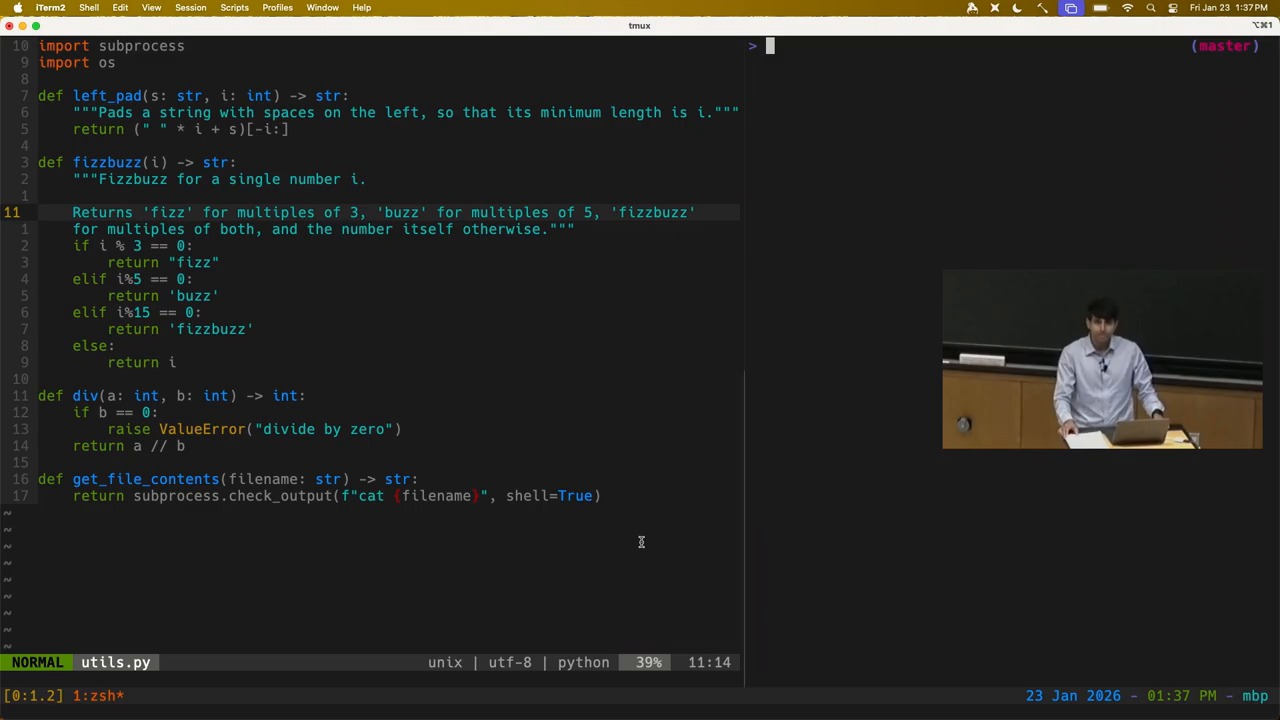
\includegraphics[width=0.92\textwidth]{figures/fig_01_minilib.jpg}
\caption{Minilib 是只有一个 Python 文件的演示库，里面是几个故意写得不太好的工具函数\vtag}
\end{figure}
\srcnote{00:01:30--00:01:45}
\end{minipage}


作为贯穿整节课的案例，讲者使用了一个他们写的小库 Minilib：一个单文件 Python 库，里面有一堆零散的工具函数，比如 \texttt{fizzbuzz} 和 \texttt{left\_pad}。这些函数本身没什么实际用处，但正好够演示这节课要讲的各种东西。讲者使用的 Python 项目管理工具是 Hatch，后面看到的 \texttt{hatch fmt}、\texttt{hatch test} 等命令都是它提供的。

\begin{knowledgebox}{本讲的工具与概念对照}
讲义作者整理：本讲的每个概念都有其他语言的对应工具。格式化：Python 的 Ruff、Black，JavaScript 的 Prettier，Go 的 gofmt；lint：Ruff、ESLint、Clippy；测试：pytest、JUnit、Rust 内置的测试框架；性质测试：Hypothesis、QuickCheck；pre-commit 钩子：pre-commit 工具或 Git 原生钩子；持续集成：GitHub Actions 等；命令运行器：just、make。记住概念，具体工具用到时再查。
\end{knowledgebox}

\section{代码格式化}

\subsection{为什么要自动格式化}

讲者说，代码自动格式化工具会自动美化程序的表层语法。用这类工具的理由是：把写代码时那些琐碎的细节、保持代码整洁的工作自动化，把脑力花在更深层、更有挑战性的问题上。他指着 Minilib 的代码说，仔细看会发现一些格式上的不一致：Python 中字符串既可以用双引号也可以用单引号，而他这里有的行用双引号、有的行用单引号；有个二元运算符两边一处有空格，另一处忘了加；可能还有其他格式化工具会发现的问题。

自动格式化工具要么检查格式是否符合标准，要么（很多工具都支持）直接修改代码使其符合标准，于是这就不再是人需要做的事了。有些工具支持多种编程语言；有些高度可配置，比如可以告诉工具“我喜欢 Python 字符串用单引号，二元运算符两边不留空格”；另一方面，也有些格式化工具的可配置性非常有限，原因是为了减少“自行车棚问题”（bikeshedding）：程序员不应该把时间花在争论单引号还是双引号好看上，而应该花在更重要的事情上。格式化工具就是设定一个标准，大家都遵守，谁都不用操心。

\begin{knowledgebox}{自行车棚问题}
讲义作者补充：bikeshedding 源自帕金森琐碎定律的一个比喻：委员会审议核电站方案时很快通过，却为自行车棚刷什么颜色争论不休，因为人人都能对简单问题发表意见。代码风格就是典型的“自行车棚”。中文课程页也用了这个术语。Black、gofmt 这类几乎不可配置的格式化工具，正是有意消灭这类争论；而 Prettier 这类可配置工具，则应把配置文件提交到版本控制中，让全组共用同一份配置。
\end{knowledgebox}

很多格式化工具还能与 IDE 集成，保存代码时自动格式化，讲者这次没有演示。

\subsection{检查模式与修复模式}

\noindent\begin{minipage}{\textwidth}
\begin{figure}[H]
\centering
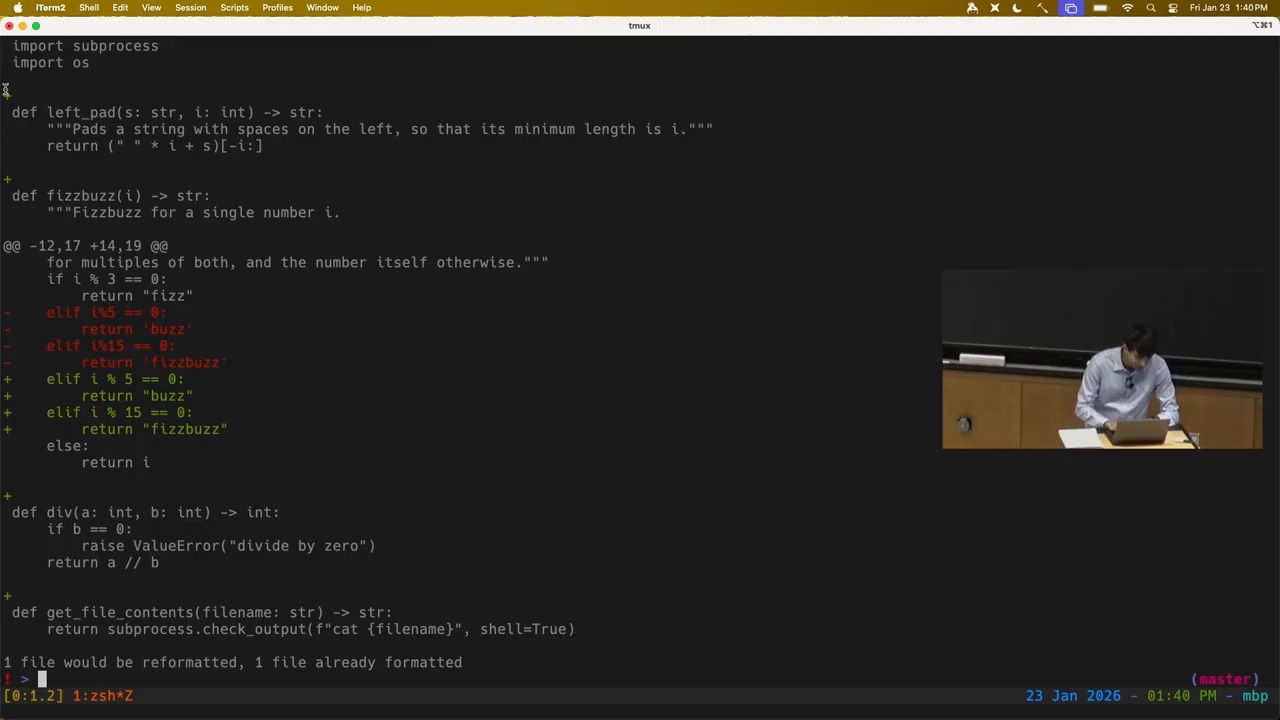
\includegraphics[width=0.92\textwidth]{figures/fig_02_fmt_check.jpg}
\caption{加上检查参数时，格式化工具只以差异形式列出它打算做的修改\vtag}
\end{figure}
\srcnote{00:04:00--00:04:15}
\end{minipage}


讲者运行 \texttt{hatch fmt -f -{}-check}，它检查代码是否符合格式标准，并显示需要修改的地方。放大窗口可以看到它显示了一个差异：函数定义之间要多留一点空行；把单引号字符串改成双引号；在二元运算符两边多加空格。讲者说他故意让这个差异保持很小。如果他再故意往参数之间加几个空格，或者在奇怪的地方加一个多余的换行，格式化工具也会修正这些；不过代码必须能被解析。

所以这些工具通常可以在只检查的模式下运行，也可以在直接修复代码的模式下运行。去掉 \texttt{-{}-check} 再运行，工具报告“1 file reformatted”；在编辑器里重新加载文件，可以看到它说要做的修改都已经做好了。

\begin{lstlisting}[language=bash]
hatch fmt -f --check   # show what the formatter would change
hatch fmt -f           # actually reformat the files
git commit -a -m "fix formatting"
\end{lstlisting}

\begin{warningbox}{这些命令是项目配置的结果}
讲义作者提醒：讲者说明 \texttt{hatch fmt} 等命令是他为这个项目配置好的，底层调用的是 Ruff，具体配置不必关心。在你自己的项目里，如果没有用 Hatch，对应的命令可能是 \texttt{ruff format}、\texttt{black .} 或 \texttt{prettier -{}-write .} 等，按所用工具的文档设置即可。
\end{warningbox}

\subsection{EditorConfig}

\noindent\begin{minipage}{\textwidth}
\begin{figure}[H]
\centering
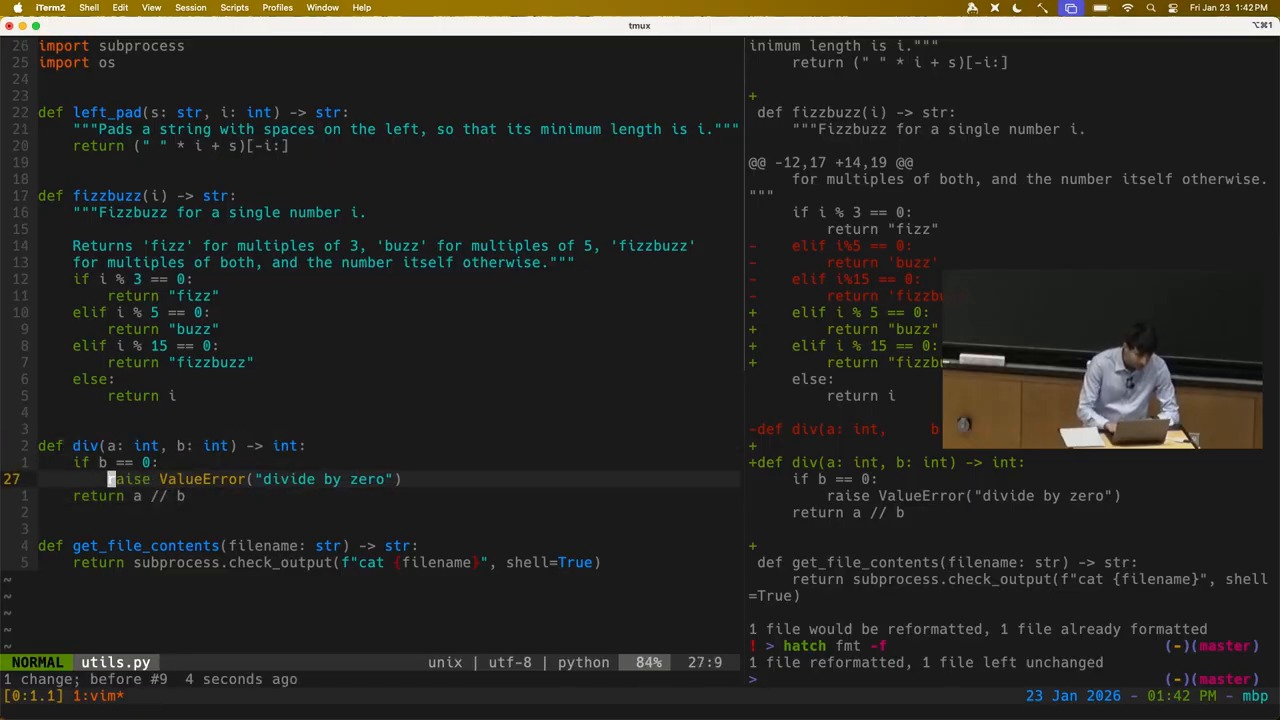
\includegraphics[width=0.92\textwidth]{figures/fig_03_editorconfig.jpg}
\caption{EditorConfig 文件放在仓库根目录，写明换行、缩进和行尾空白等编辑器设置\vtag}
\end{figure}
\srcnote{00:05:45--00:06:00}
\end{minipage}


在格式化方面，讲者还介绍了一个工具和标准：EditorConfig。它是一种文件格式加上一类 IDE 插件，帮助开发者在不同 IDE 之间保持一致的编码规范。比如你用 Vim，朋友用 VS Code，另一个朋友用 Cursor，大家在同一个代码库上工作，各人配置中的细小差异就会带来麻烦。例如缩进级别不同：讲者的 Python 代码用四个空格缩进，每按一次 Tab 缩进四个空格；但用别的缩进方式写 Python 也完全合法，有人的 IDE 可能就是那样配置的。

EditorConfig 文件放在 Git 仓库的根目录，里面有一些基本设置：文件末尾要不要有换行符？用 Tab 还是空格？编辑器是否自动删除行尾空白？讲者故意在行尾加了一堆空白，保存文件时它们就被删掉了。还可以按文件类型或文件名配置缩进大小等细节。讲者说 Missing Semester 课程的仓库就用了 EditorConfig。

\begin{lstlisting}[language=bash]
# .editorconfig (example)
root = true

[*]
end_of_line = lf
insert_final_newline = true
trim_trailing_whitespace = true

[*.py]
indent_style = space
indent_size = 4
\end{lstlisting}

讲者说代码格式化是个很简单的概念，但非常方便，他建议每个项目都用上。他随后把这些修改提交了，好让代码库在课上的现场编程中逐步变好。

\subsection{本章小结}

格式化工具处理表层语法，可以只检查，也可以直接修复；高度可配置的工具应提交配置文件，不可配置的工具用来避免风格争论；EditorConfig 让不同编辑器遵守同一套基本规则。

\section{Linter 与静态分析}

\subsection{什么是 linter}

讲者说，linter 对代码做静态分析：与动态分析相对，linter 在不运行代码的情况下分析代码，但它做的是语义分析，可以看作比只看表层语法的格式化工具更深一层。linter 试图找出代码中的反模式和潜在问题，分析深度因工具而异，但通常能在很多问题变成实际遇到的 bug 之前就把它们抓住。

\begin{importantbox}{linter 的几个要点}
\begin{itemize}
\item linter 一般自带一系列规则，以预设的形式提供，通常可以在项目层面配置。
\item 有些规则会有误报，所以很多 linter 支持按文件或按行禁用某条规则。
\item 好的 linter 有帮助文档：抱怨某段代码时，会说明它在找什么模式、为什么这种模式不好、应该避免，还可能给出更好的替代写法。
\item 有些 linter 能自动修复部分问题。但因为是语义分析，静态分析并不完美：有些规则带有“安全修复”，总是可以放心应用；有些问题虽然可能有害，却很难写出保证不改变语义、不会搞坏代码的自动变换，只能由程序员手动修复。
\end{itemize}
\end{importantbox}

\subsection{演示：检查与自动修复}

\noindent\begin{minipage}{\textwidth}
\begin{figure}[H]
\centering
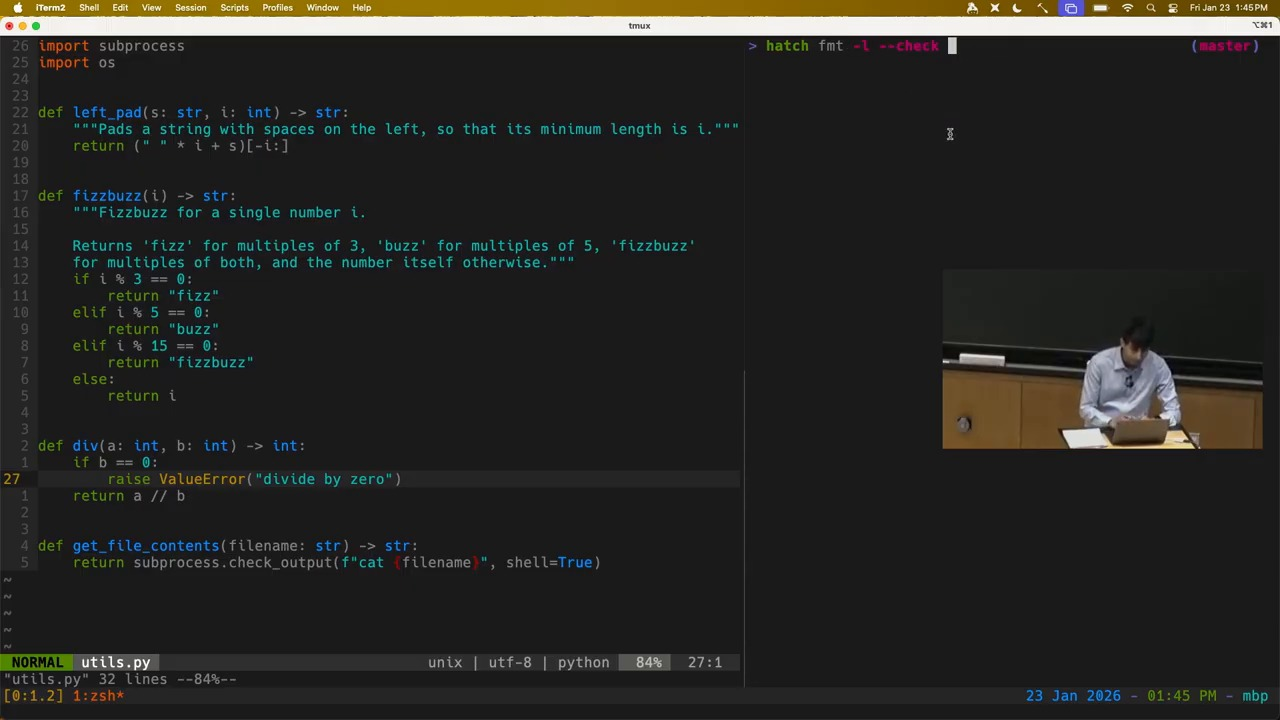
\includegraphics[width=0.92\textwidth]{figures/fig_04_lint_check.jpg}
\caption{linter 在检查模式下报告 7 个问题，并标出其中 3 个可以自动修复\vtag}
\end{figure}
\srcnote{00:09:15--00:09:30}
\end{minipage}


讲者用 Hatch 配置了一条命令来运行 linter，同样带着 \texttt{-{}-check} 只报告潜在问题。底部的汇总写着找到 7 个错误，其中 3 个可以用 \texttt{-{}-fix} 修复，另外还有一个 \texttt{-{}-unsafe-fixes} 选项，“如果你想冒险的话”。可以看到这些都是轻量的语义检查：
\begin{itemize}
\item \texttt{import *}：这会让其他静态分析更难进行，是一种反模式。
\item import 块没有排序：为了整洁，Python 的 import 最好按顺序排列。
\item 导入了没用的模块，比如 \texttt{os} 导入了但没有使用。
\item 一个 \texttt{if} 分支已经 \texttt{return}，后面却接着 \texttt{elif}：既然前一个分支会返回，后面的 \texttt{elif} 完全可以写成普通的 \texttt{if}，这也是推荐避免的模式。
\end{itemize}

这个 linter 会用星号标出可以自动修复的问题：排序 import 是安全的操作，删除未使用的导入也可以自动完成。以修复模式运行后重新加载文件，可以看到 \texttt{if/elif} 链被改成了 \texttt{if}，未使用的导入也没了。

\subsection{用 noqa 按行关闭规则}

\noindent\begin{minipage}{\textwidth}
\begin{figure}[H]
\centering
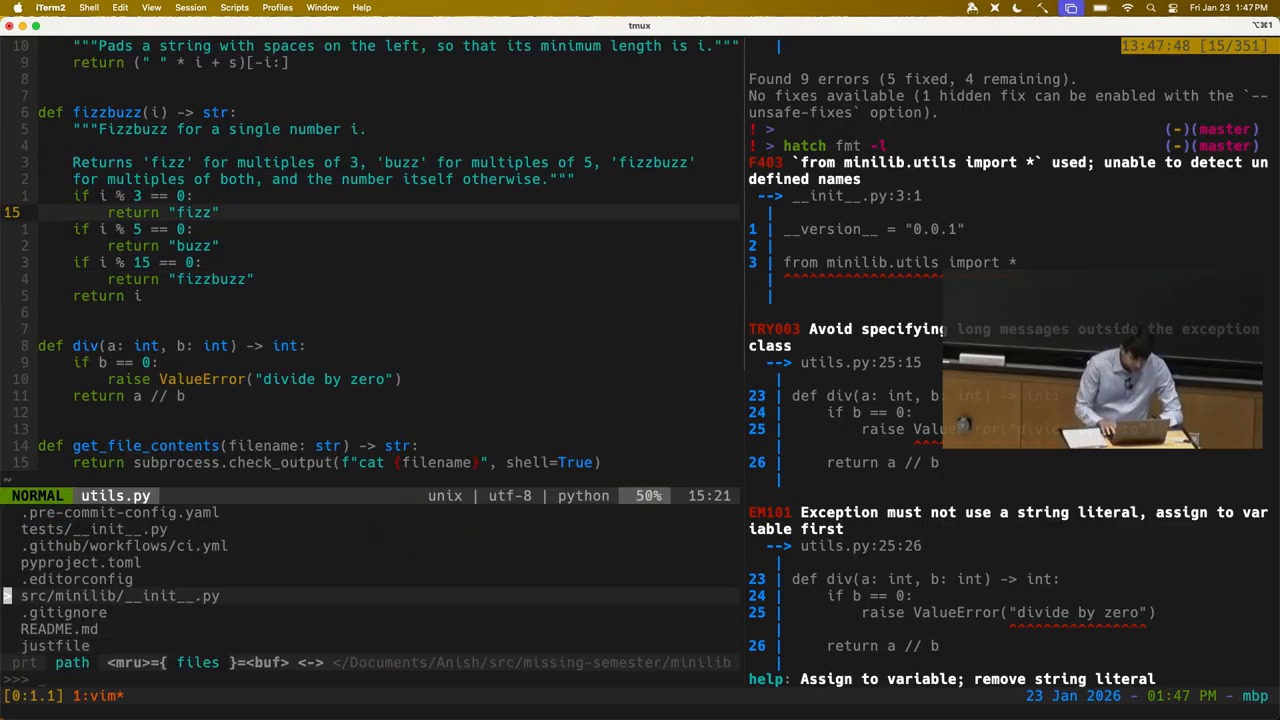
\includegraphics[width=0.92\textwidth]{figures/fig_05_lint_fix.jpg}
\caption{在行尾写上 noqa 注释和规则编号，linter 就不再报告这一行\vtag}
\end{figure}
\srcnote{00:11:30--00:11:45}
\end{minipage}


剩下的是 linter 不能自动修复的问题。第一个是 \texttt{import *}：讲者这样写，是为了能直接 \texttt{from minilib import 某个名字}，从 utils 子模块导入名字。他承认这不是好的编程实践，但为了演示，假设他就想保持这样。linter 报的是 F403 错误，于是他在这一行写上 \texttt{\# noqa: F403}，这一行的 linter 检查就被关闭了，再运行 linter，这个错误不再出现。

讲者说这就是这些工具的一般用法：尤其是大项目，你会希望保留大量静态分析，因为它们确实能帮你抓住潜在的 bug 和坏模式；但这些分析并不完美，所以可能需要在代码各处加上 \texttt{noqa} 注解。

\subsection{从 linter 文档中学习}

\noindent\begin{minipage}{\textwidth}
\begin{figure}[H]
\centering
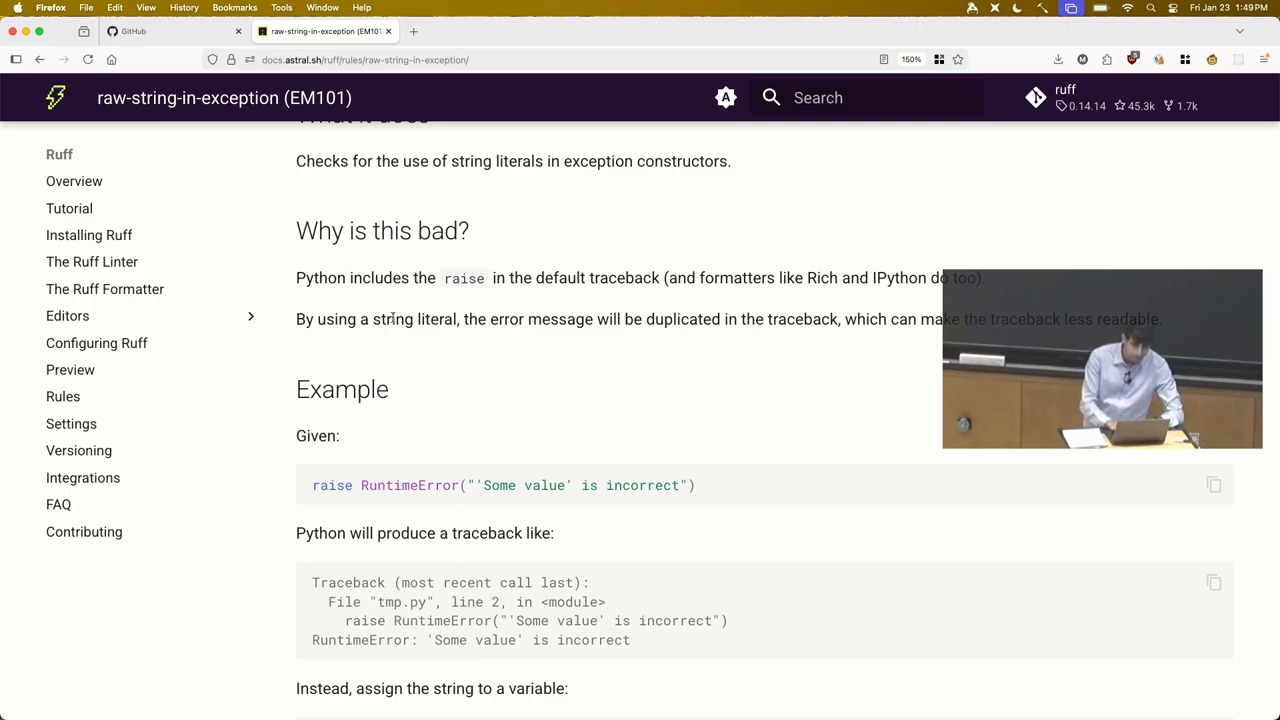
\includegraphics[width=0.92\textwidth]{figures/fig_06_ruff_doc.jpg}
\caption{Ruff 文档对每条规则都写明它检查什么、为什么不好，并给出示例\vtag}
\end{figure}
\srcnote{00:13:30--00:13:45}
\end{minipage}


讲者还想演示 linter 怎样教你写更好的代码。第二个问题是一段代码抛出 \texttt{ValueError}，里面直接写了一个字符串字面量“divide by zero”。linter 报告 EM101：异常不能直接使用字符串字面量，要先赋值给变量。这告诉了我们怎么做，可以直接去改；但如果想知道为什么不好，可以搜一下。他用的 linter 底层是 Ruff，Ruff 有详尽的文档解释每一条规则：它做什么、在找什么模式，以及为什么不好。

文档解释说：Python 中执行 raise 语句时会显示回溯，即导致这个异常的那些代码行，下面还会显示错误信息。如果在 raise 这一行直接写字符串字面量，信息就会出现两次：一次在回溯里显示的那行代码中，一次在最后的错误类和错误信息中，既冗余又占屏幕。修正方法是多写一行，先把字符串绑定到变量，这样回溯中就只看到 \texttt{raise RuntimeError(msg)}，没有重复的字符串。

\begin{lstlisting}[language=Python]
# Flagged by EM101: the message appears twice in the traceback
raise ValueError("divide by zero")

# Preferred: bind the message to a variable first
msg = "divide by zero"
raise ValueError(msg)
\end{lstlisting}

\subsection{shell=True 的安全隐患}

修好之后再运行 linter，只剩一个问题：代码用 Python 的 \texttt{subprocess} 模块调用 \texttt{cat} 命令，但带了 \texttt{shell=True}。这样不是直接调用 \texttt{cat} 程序，而是调用讲者电脑上的 shell（Z Shell），由它解析字符串并执行。讲者说这有潜在的安全问题，简单说就是：如果文件名里含有某些奇怪的字符，比如分号后面跟着别的东西，分号后面的部分就会被 shell 当作代码执行。这是应该避免的坏模式，这条 linter 规则能抓住它。

讲者说实践中你应该直接修掉它，但他想先暂时用 \texttt{\# noqa: S602} 压下这条，因为接下来要用它介绍另一个工具。加上之后再运行，linter 不再返回非零退出码，而是显示“All checks passed”并返回 0。

\begin{warningbox}{不要把 noqa 当作修复}
讲义作者提醒：讲者压下 S602 只是为了演示后面的 semgrep，他明确说实践中应当修复。正确的做法是不经过 shell，直接传参数列表，例如 \texttt{subprocess.check\_output(["cat", filename])}，这样文件名中的分号等字符不会被解释为命令。\texttt{noqa} 只应用于确认是误报、或有意为之并能说明理由的地方，最好在旁边写注释解释原因。
\end{warningbox}

\subsection{自定义规则：semgrep}

\noindent\begin{minipage}{\textwidth}
\begin{figure}[H]
\centering
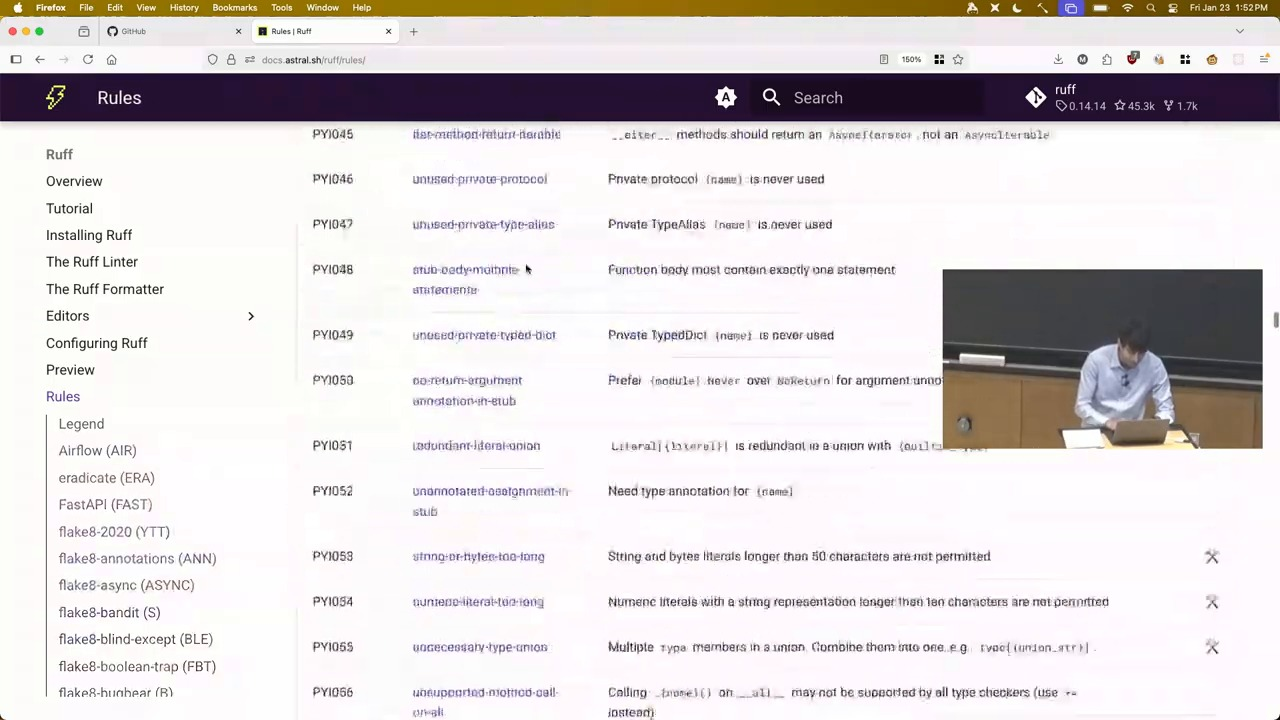
\includegraphics[width=0.92\textwidth]{figures/fig_07_ruff_rules.jpg}
\caption{Ruff 的规则列表很长，覆盖数百种代码模式\vtag}
\end{figure}
\srcnote{00:16:00--00:16:15}
\end{minipage}


讲者说，给项目配置 linter 时，一般会选所用语言的某个流行工具，它会带一大串内置规则。比如 Ruff 有 800 种它会在代码中查找的模式，还有一个巨大的列表逐一解释。这对入门很好；但有时具体项目需要项目特定的规则，比如某个项目规定不用 Python 的 \texttt{pickle} 模块，因为它可能被不安全地使用；或者不允许代码使用 Python 的 \texttt{exec} 函数。这时能编写自己的 linter 规则就很方便。有时主 linter 工具本身可配置，但另一个很有用的工具是 semgrep，意思是“语义 grep”（semantic grep）。

\noindent\begin{minipage}{\textwidth}
\begin{figure}[H]
\centering
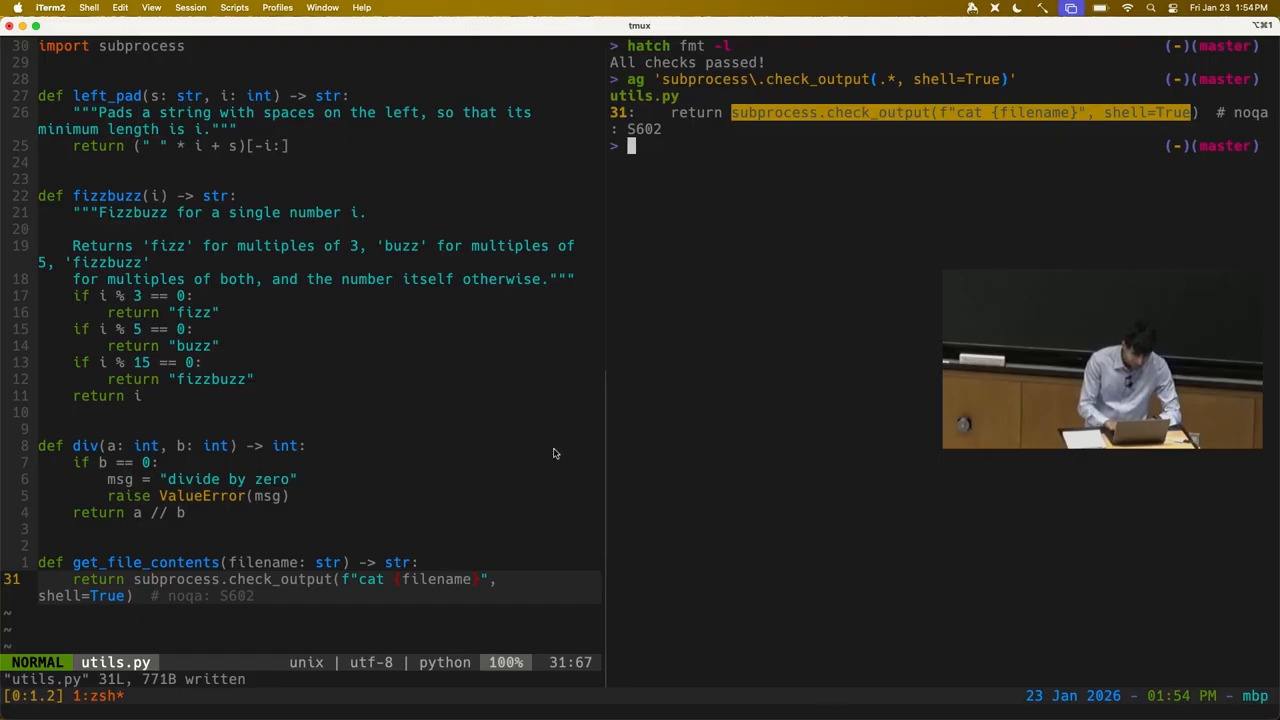
\includegraphics[width=0.92\textwidth]{figures/fig_08_ag_regex.jpg}
\caption{用正则表达式搜索 shell=True 的调用，模式写得很脆弱\vtag}
\end{figure}
\srcnote{00:17:45--00:18:00}
\end{minipage}


第一讲介绍过 grep，它在文本或代码中搜索字符串模式。semgrep 概念上类似，但它会解析所用编程语言的语法树，在那个层面上搜索，所以比字符层面的语法搜索更深入。讲者举例：假设 linter 没有内置检查 \texttt{subprocess.check\_output} 带 \texttt{shell=True} 的规则，可以用 grep 的替代品 \texttt{ag} 写一个正则表达式来搜，比如 \texttt{subprocess.check\_output}、括号、\texttt{.*}（正则中表示任意数量的字符）、逗号、\texttt{shell=True}。搜索确实匹配到了那一行，于是可以写个小脚本在项目中查找这类坏模式。

问题是这个正则表达式很脆弱。讲者先发现括号在正则中是捕获组，不是字面括号，改正之后，只要给 \texttt{check\_output} 再加一个关键字参数，模式就不匹配了；把调用拆成多行（Python 完全允许这样写，虽然格式化工具大概会改回去）也会让它失配，因为内容分布在多行上。你可以花很多力气打地鼠一样写一堆正则去覆盖各种情况，但更好的办法是用 semgrep。

\noindent\begin{minipage}{\textwidth}
\begin{figure}[H]
\centering
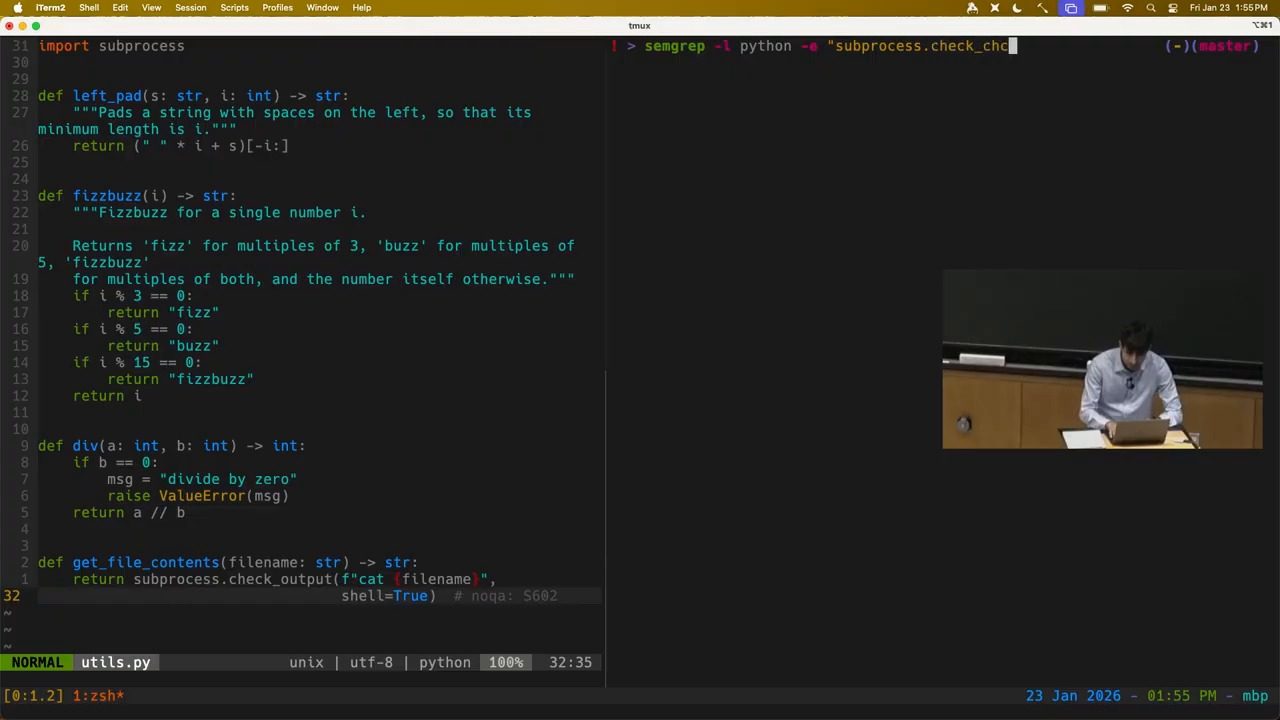
\includegraphics[width=0.92\textwidth]{figures/fig_09_semgrep.jpg}
\caption{semgrep 理解 Python 语法，即使调用跨行也能匹配出来\vtag}
\end{figure}
\srcnote{00:19:00--00:19:15}
\end{minipage}


semgrep 是语言感知的：可以告诉它“在 Python 程序中搜索这个模式”：查找 subprocess 模块中 \texttt{check\_call} 或 \texttt{check\_output} 的所有调用，参数中有一些参数、然后是 \texttt{shell=True}、然后是更多参数。运行后，即使调用中有换行，它也能找到；再加别的参数，依然匹配。讲者说，semgrep 是编写自定义轻量分析、增强项目 linter 的有用工具。

\begin{lstlisting}[language=bash]
# Fragile: text-level search breaks on line breaks or extra arguments
ag 'subprocess.check_output\(.*, shell=True'

# Robust: semgrep matches on the Python syntax tree
semgrep -l python -e 'subprocess.check_output(..., shell=True, ...)'
\end{lstlisting}

\begin{knowledgebox}{为什么语法树层面更可靠}
讲义作者补充：文本层面的搜索看到的是字符序列，换行、空格、参数顺序和注释都会改变字符序列；语法树层面的搜索看到的是“一个函数调用，函数名是什么，参数里有没有某个关键字参数”，与排版无关。semgrep 模式中的 \texttt{...} 表示任意数量的参数，比正则中的 \texttt{.*} 语义清晰得多。中文课程页给出的例子是用同样的方式查找 \texttt{subprocess.Popen(..., shell=True, ...)}。
\end{knowledgebox}

演示中还出了个小插曲：讲者把调用拆成多行后，原来写在行尾的 \texttt{noqa} 注释失效了，他重新放好位置才让 linter 通过，然后提交了修改。

\subsection{本章小结}

linter 做不运行代码的语义检查，能自动修复其中安全的部分；误报可以用 \texttt{noqa} 按行关闭；规则文档是学习好写法的好材料；项目特定的规则可以用 semgrep 在语法树层面编写，比正则表达式可靠。

\section{软件测试}

\subsection{测试的层次与方法}

讲者说测试是个很深的话题，可以讲好几节课，这里只介绍一些高层概念，鼓励大家课后自己探索。软件测试是提高对所写代码信心的标准技术，基本思想是：写一些代码，再写一些代码去调用刚才的代码，检查它是否按预期运行。测试的价值是长期的：随着代码演化，可以一直运行测试，确保没有东西被搞坏。

\begin{knowledgebox}{测试的粒度}
讲者按粒度区分了几类测试：
\begin{itemize}
\item 单元测试：测试单个函数，比如“fizzbuzz 应该这样表现，left\_pad 应该那样表现”。
\item 集成测试：测试项目中不同模块或服务之间的交互。
\item 功能测试：更偏端到端，检查软件是否满足用户需求，可以评估完整的端到端场景。
\end{itemize}
他说讲义里写了这些，人们还发明了很多其他术语来描述不同的测试方法，这是一个很深的领域。
\end{knowledgebox}

测试方法也有很多。一种流行的开发方式叫测试驱动开发（TDD）：不是先写实现再补测试，而是反过来：你对要实现的东西有一个想法、心里有一个规格，先把这个规格（或部分规格）表达为测试，即“我要写的这个函数应该这样表现”，然后再写实现，运行测试确认实现满足规格。

\subsection{用 pytest 写第一个测试}

讲者说，盯着左边代码看的同学可能已经发现了一些 bug，这次从测试的角度出发，写测试来帮我们抓住这些 bug。先给 \texttt{fizzbuzz} 写测试：他把 FizzBuzz 改成了一个函数，规格用英文写着：对给定整数 $i$，3 的倍数返回 Fizz，5 的倍数返回 Buzz，同时是 3 和 5 的倍数返回 FizzBuzz，否则返回数字本身。

讲者说，测试框架的具体设置、测试放在哪里，取决于编程语言和测试框架。他用的是 Python 和 pytest；在自己的项目中到了这一步，查一下所用语言该怎么设置测试即可。在 pytest 中，测试放在特定位置，函数名以 \texttt{test\_} 开头，就是不带参数、没有返回值、里面全是 \texttt{assert} 语句的普通 Python 函数，测试框架会在你要求时运行所有这些函数。

\noindent\begin{minipage}{\textwidth}
\begin{figure}[H]
\centering
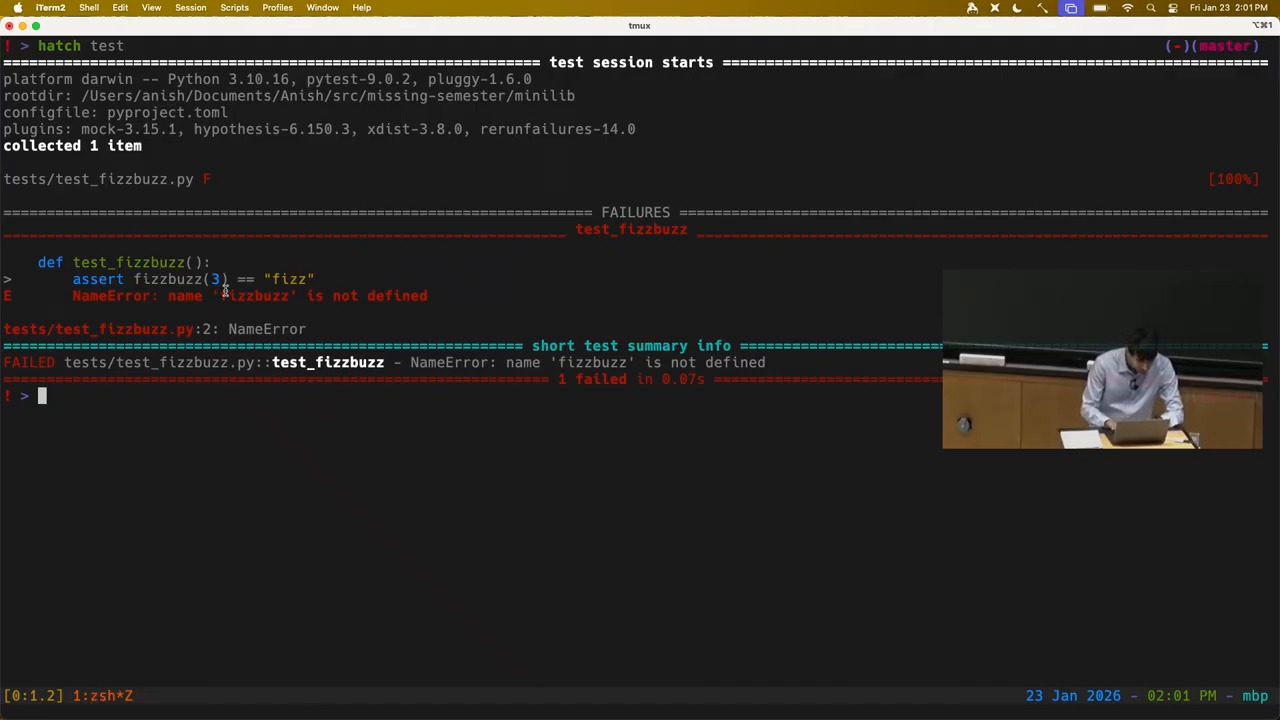
\includegraphics[width=0.92\textwidth]{figures/fig_10_pytest_first.jpg}
\caption{第一次运行测试就报名字未定义，原来是测试文件忘了导入被测模块\vtag}
\end{figure}
\srcnote{00:25:00--00:25:15}
\end{minipage}


他写下 \texttt{assert fizzbuzz(3) == "Fizz"}，用 \texttt{hatch test} 运行，结果报 NameError：\texttt{fizzbuzz} 未定义。讲者说这也说明测试本身也可能有 bug：他忘了导入模块。加上 \texttt{from minilib import fizzbuzz} 再运行，全绿，一个测试通过。

\noindent\begin{minipage}{\textwidth}
\begin{figure}[H]
\centering
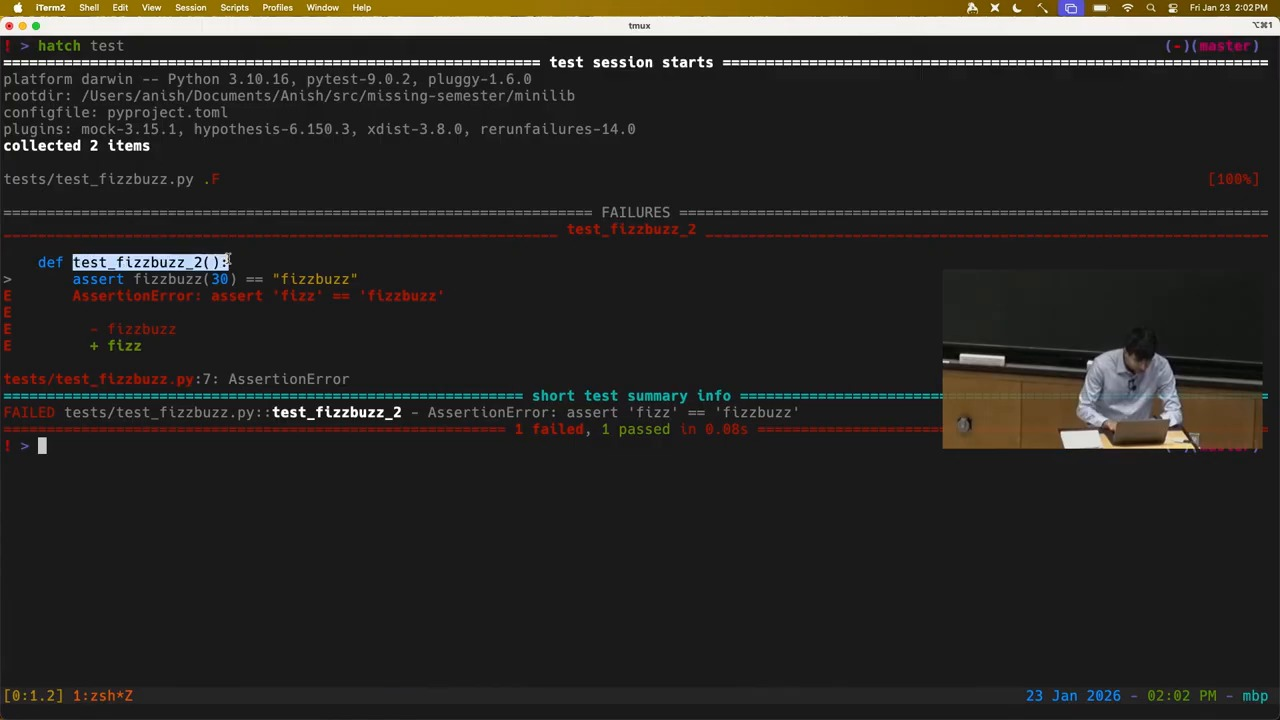
\includegraphics[width=0.92\textwidth]{figures/fig_11_pytest_fail.jpg}
\caption{fizzbuzz(30) 的测试失败，断言显示实际返回值与期望值不同\vtag}
\end{figure}
\srcnote{00:25:45--00:26:00}
\end{minipage}


再加一个测试：\texttt{fizzbuzz(30)} 应该是 \texttt{"FizzBuzz"}。运行后测试失败，断言错误显示左边实际返回的是 \texttt{"Fizz"}，而期望是 \texttt{"FizzBuzz"}。有了这个失败，就可以分析代码：对这个具体输入，为什么没有得到预期的具体输出？讲者发现，检查 15 的倍数的分支应该放在最前面。改好后再运行，两个测试都通过了。

\begin{lstlisting}[language=Python]
from minilib import fizzbuzz

def test_fizzbuzz_1():
    assert fizzbuzz(3) == "Fizz"

def test_fizzbuzz_2():
    assert fizzbuzz(30) == "FizzBuzz"
\end{lstlisting}

\subsection{代码覆盖率}

讲者接着问：怎样衡量测试写得好不好？部分答案是：很难写一个程序告诉你测试好不好，因为这需要创造力，你需要以正确的方式去调用代码。测试有点像一门手艺，会随时间越做越好。但有些工具能帮忙，比如代码覆盖率（code coverage）这个指标：看实现中有哪些代码行真正被测试执行到了。

\noindent\begin{minipage}{\textwidth}
\begin{figure}[H]
\centering
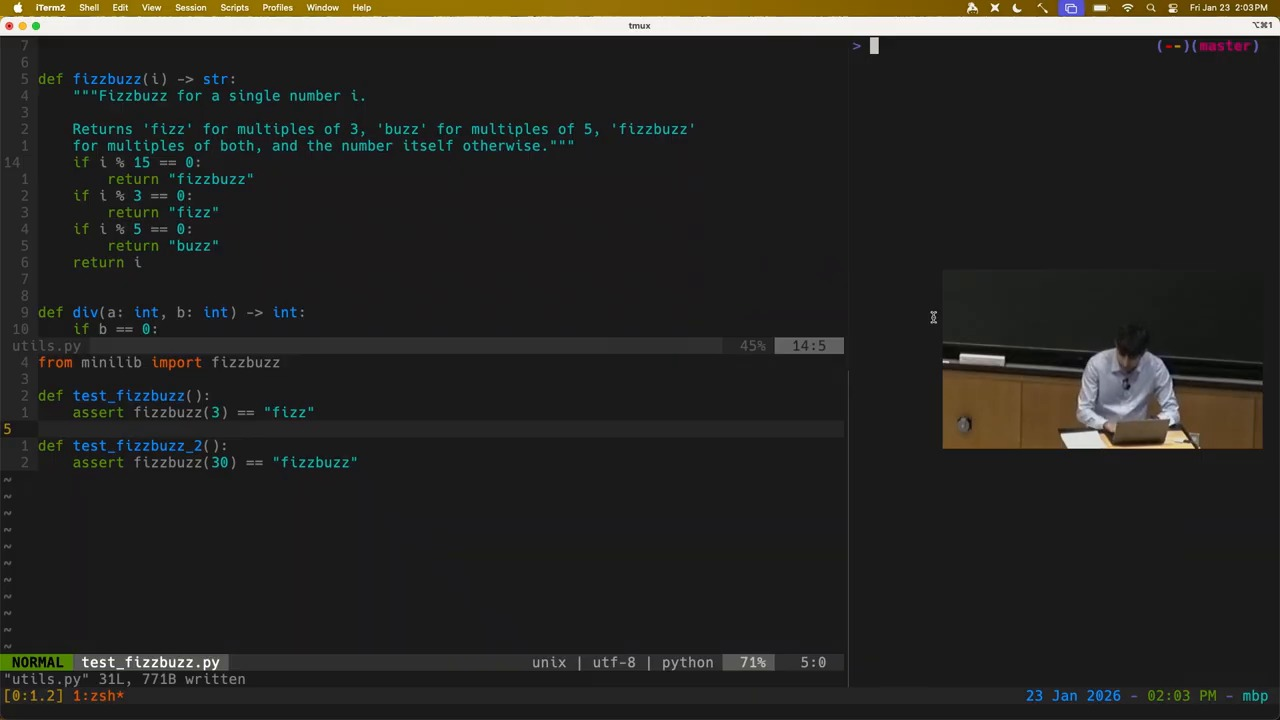
\includegraphics[width=0.92\textwidth]{figures/fig_12_coverage_term.jpg}
\caption{带覆盖率运行测试，终端汇总显示 18 条语句中有 9 条未被执行\vtag}
\end{figure}
\srcnote{00:27:00--00:27:15}
\end{minipage}


讲者用 \texttt{hatch test -c} 运行测试并计算覆盖率，结果显示 \texttt{utils.py} 有 18 条语句，漏掉了 9 条，覆盖率只有 50\%，实现中有很多代码没有被测试到。

\noindent\begin{minipage}{\textwidth}
\begin{figure}[H]
\centering
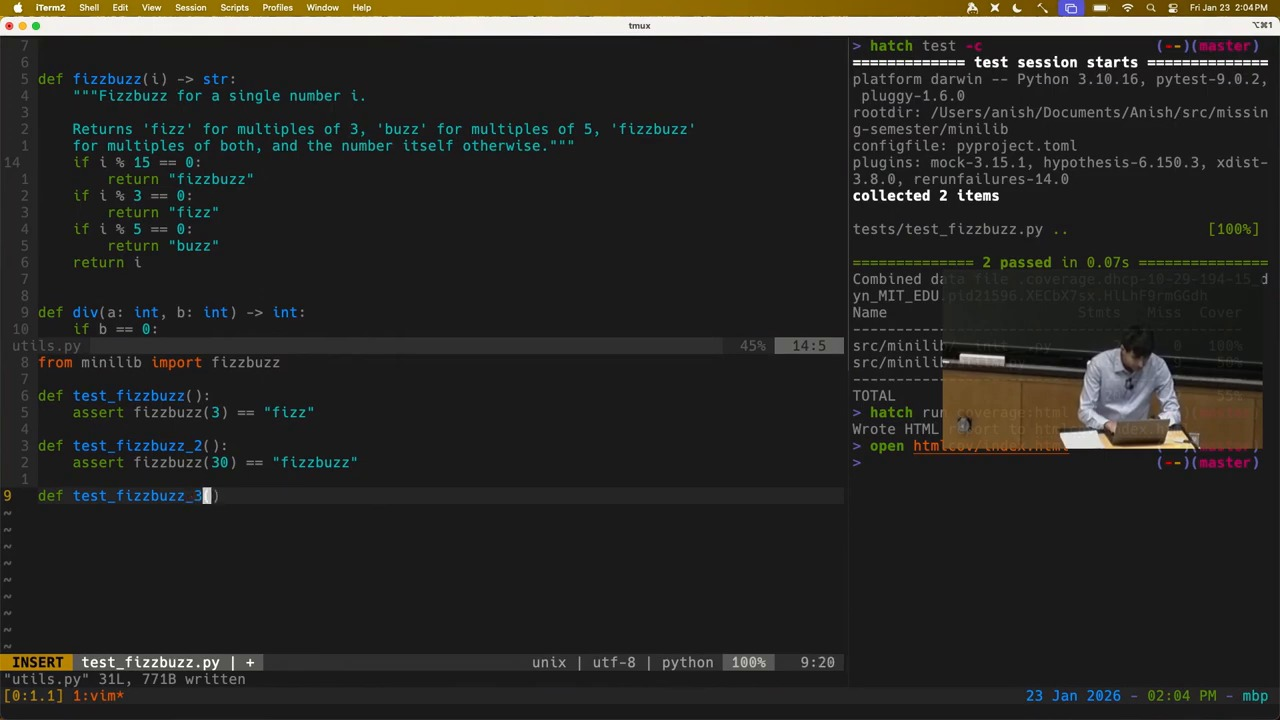
\includegraphics[width=0.92\textwidth]{figures/fig_13_coverage_html.jpg}
\caption{HTML 覆盖率报告用颜色区分哪些代码行被测试执行过\vtag}
\end{figure}
\srcnote{00:28:15--00:28:30}
\end{minipage}


覆盖率工具还能生成更好看的报告：\texttt{hatch run coverage html} 生成一份 HTML 报告，可以在浏览器中打开，帮你看清写测试时该关注哪里。打开 \texttt{utils.py} 可以看到：\texttt{i = 30} 的那个测试覆盖到的行是白色（无底色）的，第一个测试覆盖的行也是；但另外两个分支没有被覆盖，下面的一些代码也没有。

于是他补了一个测试 \texttt{fizzbuzz(99)}，应该返回 Fizz。重新运行后发现没什么用，因为 3 的倍数已经测过了；要覆盖的是那个 Buzz 分支，所以改成 \texttt{fizzbuzz(95)}，应该返回 Buzz。再带覆盖率运行，覆盖率升到了 61\%（原先是 50\%），HTML 报告里那一行也变成已覆盖。

\begin{importantbox}{覆盖率是有用但不完美的指标}
讲者认为代码覆盖率是一个相当不错的指标，评估网上找到的开源项目时也值得看一看：如果他们认真运行这些代码质量工具，多半也会在意覆盖率；如果一个项目覆盖率很低，你就无从判断代码质量如何。但覆盖率并不完美：对于更复杂的代码，完全可以写出覆盖率很高、却没什么意义的测试，它们并没有真正充分地检验程序，软件可能带着 bug 通过所有测试。
\end{importantbox}

\subsection{用 AI 提高覆盖率}

有同学问能不能用 AI 帮忙提高覆盖率。讲者说完全可以，这也是本讲推荐的习题之一：可以搭一个闭环，让 AI 智能体能够运行测试、带覆盖率运行并生成报告，可以是 HTML 格式，或者用他这个工具生成的 XML 格式报告，后者更紧凑，可能更适合交给 LLM；然后告诉它“提高覆盖率，直到 100\%”。AI 编程智能体写测试其实相当不错。

但要记住，覆盖率不是完美指标，AI 写测试也不完美。讲者说他见过 AI 生成测试的仓库，尤其是前端，覆盖率 100\%，测试却几乎完全没用。有同学问能否引导 AI 去“测试功能”，讲者说可以，AI 写测试可以相当好，只是不一定完美，要仔细审查它的产出；有时需要给它更多输入，而不只是“给我的程序写测试”，要引导它，才能产出更好的测试。

课程最后的答疑中，讲者现场演示了这个过程：用一段两三句话的简短提示，让智能体写测试、复现 bug、修复 bug、调整测试，反复迭代直到收敛，覆盖率达到 100\%。由于这些函数很简单，生成的测试相当不错：测试了 3、5、15 的各种倍数，覆盖了 fizzbuzz 的所有情况，也测试了异常是否被正确抛出。Jon 补充说，一开始 AI 会给出很有用的测试，但让它生成得越来越多，它就会开始生成没用的测试，除非你好好引导；协作起来，才能达到很好的效果。

\begin{practicebox}{让智能体补测试}
讲义作者整理：在一个有测试的小项目里，先自己运行一次带覆盖率的测试，记下覆盖率；然后让编程智能体在能运行测试和覆盖率工具的环境中补测试，要求它说明每个新测试检验的是哪条行为。完成后逐个阅读新测试，删掉只为执行代码行、却没有有意义断言的测试，再比较删除前后的覆盖率。
\end{practicebox}

\subsection{本章小结}

测试按粒度分为单元、集成、功能测试；pytest 的测试就是以 \texttt{test\_} 开头、包含断言的普通函数；失败的测试给出具体的反例，帮助定位 bug；覆盖率告诉你哪些代码没被测到，但高覆盖率不等于好测试，AI 写的测试尤其需要审查。

\section{性质测试}

\subsection{从具体用例到性质}

讲者问大家有没有发现 \texttt{left\_pad} 函数的 bug：它有一个 bug，但因为写法很绕，不太容易发现。\texttt{left\_pad} 的规格是：给定一个字符串，在左边补空格，使其最小长度为 $i$，这在命令行程序中做表格格式化时很有用。

借此他介绍另一种测试方法：性质测试（property-based testing）。不是写离散的测试用例（给定这个具体输入，程序是否产生这个具体输出），而是写下函数应该具有的性质，由测试库自动生成大量输入去检验这些性质。这让你更接近为程序写下形式化规格：它们通常不是完整的规格，但可以写下应当成立的部分规格。

他用的是 Python 的 Hypothesis 库。讲者说这种方法最初由 Haskell 的 QuickCheck 库发明和推广，现在很多编程语言都有支持它的库。

\subsection{写下 left\_pad 的性质}

讲者让大家“戴上数学帽子”，给出形如“对所有字符串 $s$、所有整数 $i$，某性质成立”的陈述。有同学提出输出长度等于 $i$，讲者说很接近：规格是输出的最小长度为 $i$，如果字符串长度为 5、$i$ 也是 5，输出就是长度 5；而如果原字符串比 $i$ 长，结果比 $i$ 长也没关系，只是永远不应短于 $i$。所以第一条性质是：对所有 $s$ 和 $i$，\texttt{len(left\_pad(s, i)) >= i}。

\noindent\begin{minipage}{\textwidth}
\begin{figure}[H]
\centering
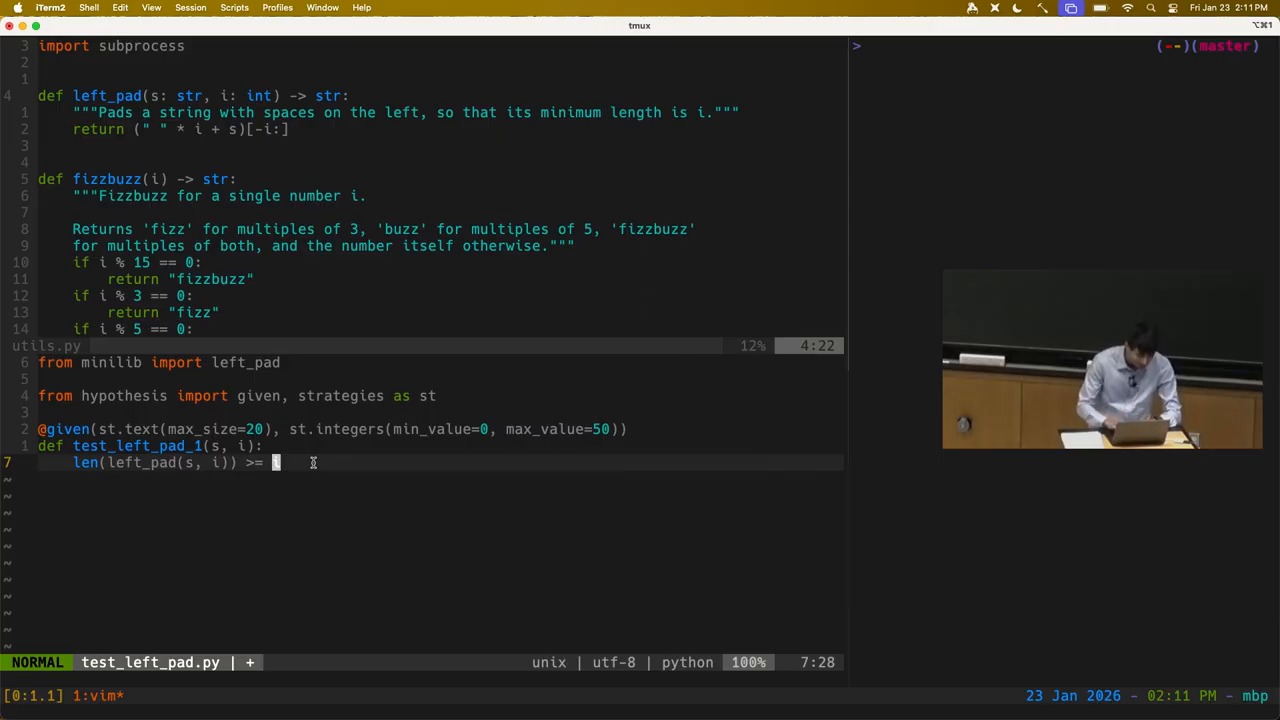
\includegraphics[width=0.92\textwidth]{figures/fig_14_hypothesis.jpg}
\caption{用 Hypothesis 写下两条性质，并限定生成输入的范围\vtag}
\end{figure}
\srcnote{00:35:30--00:35:45}
\end{minipage}


讲者强调，Hypothesis 并不是在对性质做数学证明（确实有一些技术可以对代码做这种很深的推理），它做的是生成一堆随机输入，看性质是否成立。所以需要参数化、给它一点帮助：比如 $s$ 考虑长度不超过 20 的文本，$i$ 考虑 0 到 50 之间的整数，这需要一点人的直觉。第二条性质是：补齐之后，原字符串应该包含在结果中。

\begin{lstlisting}[language=Python]
from hypothesis import given
from hypothesis import strategies as st
from minilib import left_pad

@given(st.text(max_size=20), st.integers(min_value=0, max_value=50))
def test_left_pad_1(s, i):
    assert len(left_pad(s, i)) >= i

@given(st.text(max_size=20), st.integers(min_value=0, max_value=50))
def test_left_pad_2(s, i):
    assert s in left_pad(s, i)
\end{lstlisting}

\subsection{部分规格与反例}

两条性质都通过了。讲者想重现他前一天凌晨两点写进去的那个 bug，但想不起来了，于是干脆故意改坏实现：比如让填充长度乘以 $i$ 再加上 $s$。这显然是错的，但它仍然满足这两条性质。讲者说这正好展示了性质测试的另一面：它是部分规格，只检查某些性质是否成立，而这个错误的实现恰好满足它们。他又试了直接返回 $s$，也满足第二条；再改成取子串，结果测试居然还是通过了。

现场排查后发现，原来是他测试里忘了写 \texttt{assert}：表达式只是被求值，真假都不影响，然后继续执行下一行。讲者说这又是一个测试本身有 bug 的例子。补上 \texttt{assert} 之后，第一条性质对这个坏代码依然成立，但第二条（原字符串包含在结果中）不再成立。

\noindent\begin{minipage}{\textwidth}
\begin{figure}[H]
\centering
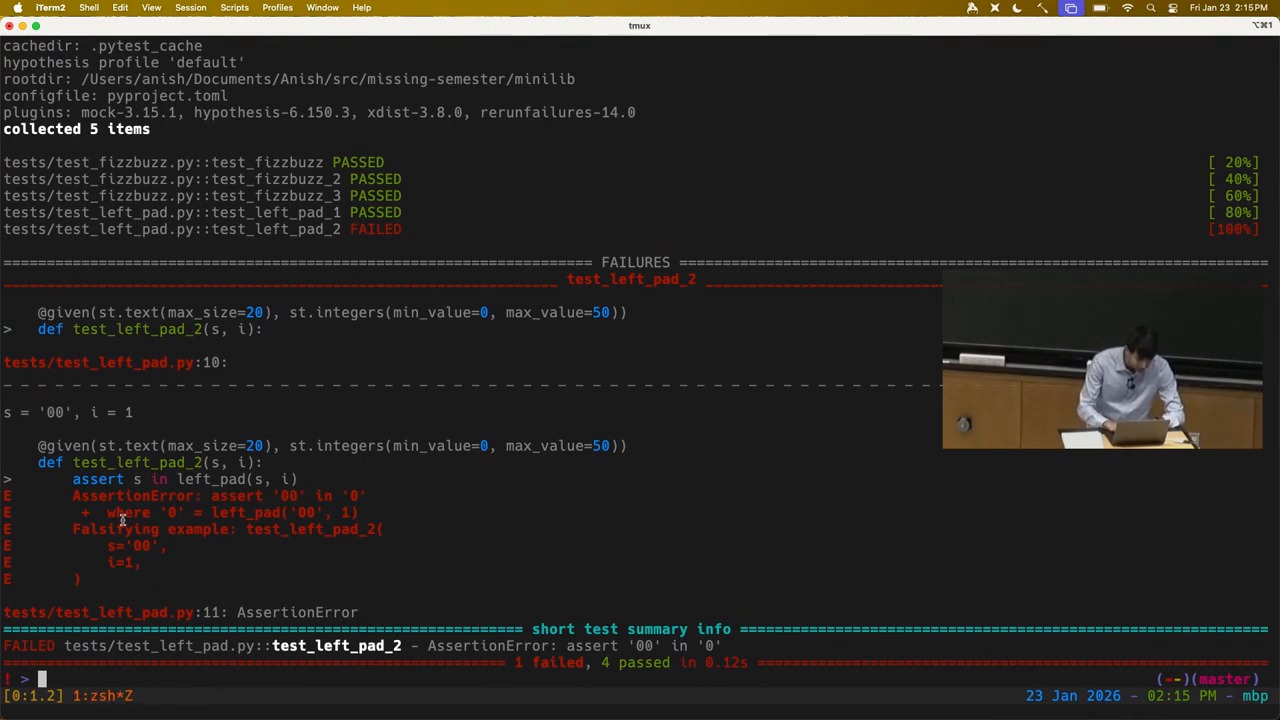
\includegraphics[width=0.92\textwidth]{figures/fig_15_counterexample.jpg}
\caption{Hypothesis 找到一个具体的反例：两个字符的字符串配上很小的长度\vtag}
\end{figure}
\srcnote{00:39:15--00:39:30}
\end{minipage}


性质测试的妙处在于：它在大量随机输入上尝试，然后给出一个性质不成立的具体反例，这里是 $s$ 为字符串 \texttt{"00"}、$i$ 为 1。有了具体的反例，就可以去调试代码。讲者出于时间考虑没有现场修复，留给有兴趣的同学自己去修，让它通过这些性质测试。

\begin{warningbox}{忘写 assert 的测试永远通过}
讲义作者提醒：讲者的现场插曲值得记住。一个只写了 \texttt{len(left\_pad(s, i)) >= i} 而没有 \texttt{assert} 的测试函数，无论结果真假都会“通过”。检查测试是否真的有效的一个简单办法，是故意把实现改坏，确认测试会失败；如果改坏了测试仍然全绿，问题可能在测试本身。
\end{warningbox}

\begin{knowledgebox}{性质测试中的“收缩”}
讲义作者补充：Hypothesis 和 QuickCheck 在找到失败输入后，会自动尝试把它“收缩”（shrink）成更简单的输入，所以报告出来的反例通常很短，比如这里的 \texttt{"00"} 和 1，而不是一串随机字符。这让反例更容易拿去调试，也是性质测试比手写随机测试更好用的原因之一。
\end{knowledgebox}

\subsection{本章小结}

性质测试写下“对所有输入都应成立”的部分规格，由库自动生成输入并给出最小化的反例；它不是证明，生成范围需要人来设定；部分规格可能被错误实现满足，所以要选择足够有区分力的性质。

\section{pre-commit 钩子}

讲者说，另一个能在所有贡献者之间强制代码质量的工具是 pre-commit 钩子：一种设置 Git 在每次提交之前运行脚本的机制。这个项目已经配置好了格式化工具、linter 和运行测试的方法。

\noindent\begin{minipage}{\textwidth}
\begin{figure}[H]
\centering
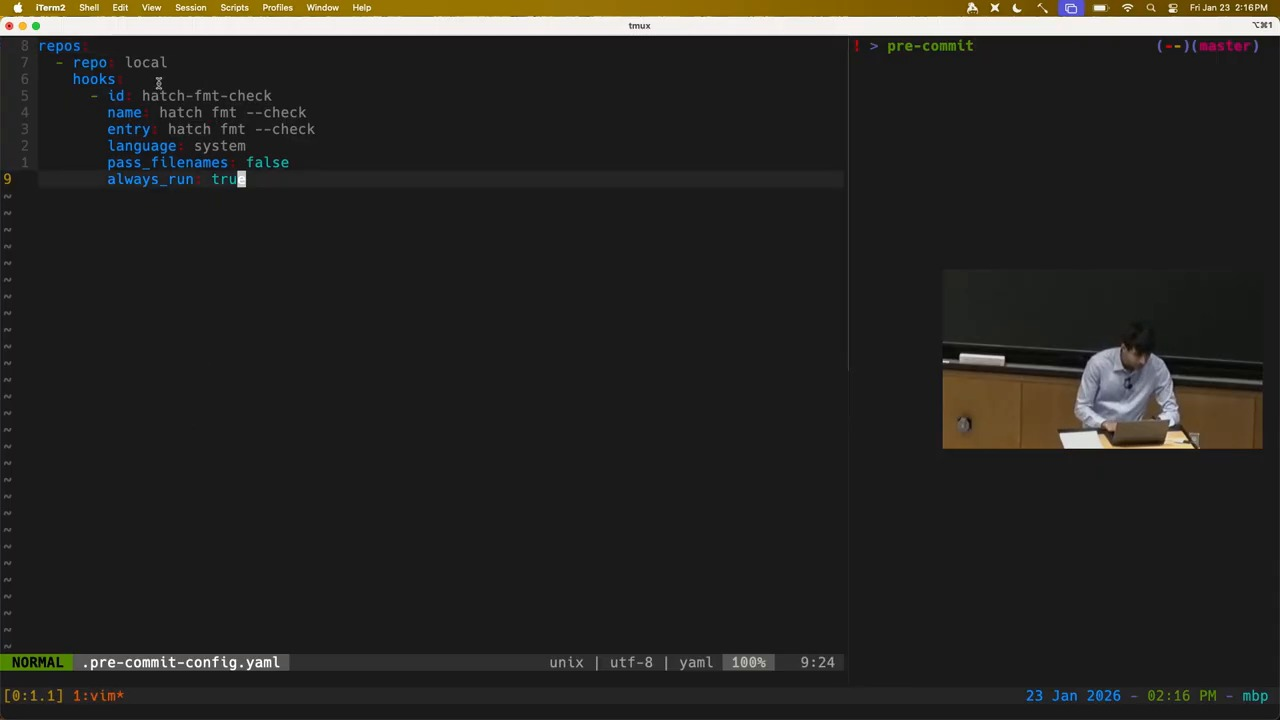
\includegraphics[width=0.92\textwidth]{figures/fig_16_precommit_cfg.jpg}
\caption{pre-commit 配置文件指定提交前要运行的检查命令\vtag}
\end{figure}
\srcnote{00:40:30--00:40:45}
\end{minipage}


在 \texttt{.pre-commit-config.yaml} 文件中，他配置了一个叫 pre-commit 的程序（讲义中有链接；pre-commit 钩子本身也是一个通用概念），让它在任何提交之前运行 \texttt{hatch fmt -{}-check}。在这个仓库上工作的开发者只需要运行一次 \texttt{pre-commit install}，它就会把钩子安装到 Git 目录中。

\noindent\begin{minipage}{\textwidth}
\begin{figure}[H]
\centering
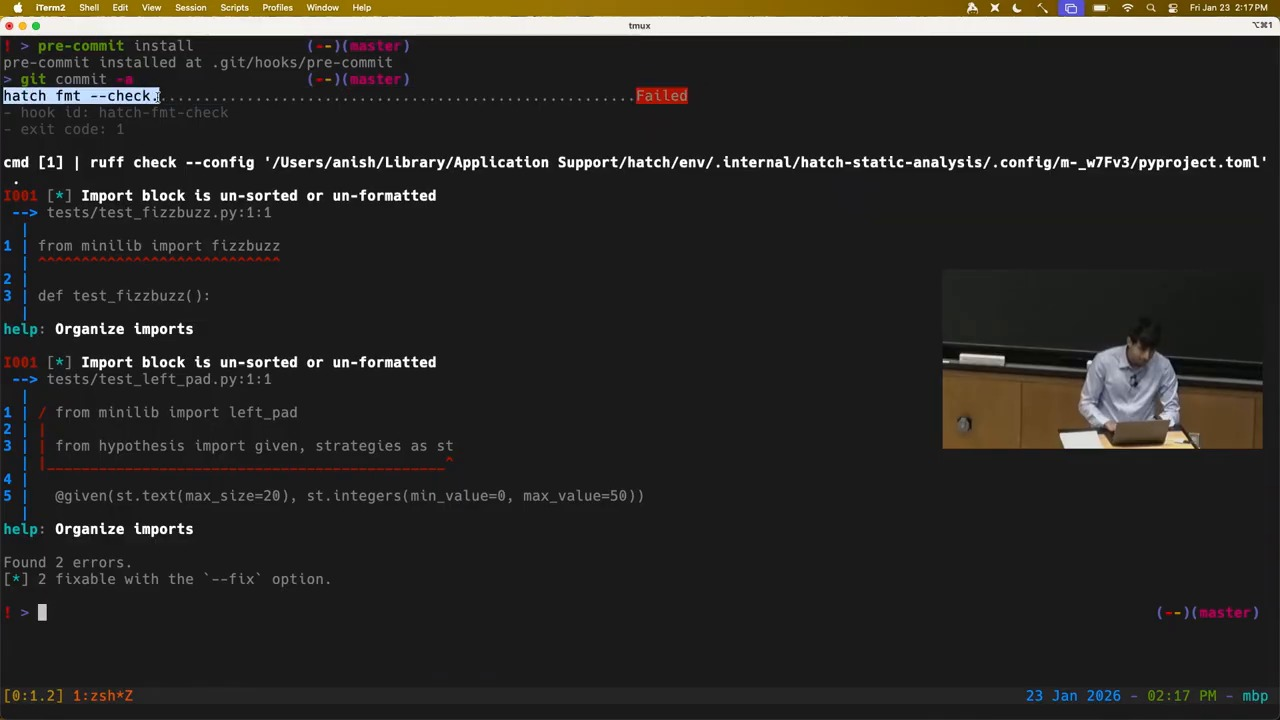
\includegraphics[width=0.92\textwidth]{figures/fig_17_precommit_fail.jpg}
\caption{格式检查失败时，pre-commit 会阻止提交并打印出问题所在\vtag}
\end{figure}
\srcnote{00:41:00--00:41:15}
\end{minipage}


之后如果代码有问题，比如讲者故意把格式弄乱再执行 \texttt{git commit}，在弹出编辑器让你写提交信息之前，所有 pre-commit 钩子都会先运行。这里 \texttt{hatch fmt -{}-check} 返回了非零退出码，pre-commit 和 Git 将其解释为出错，并显示调试输出；在修好这些问题之前，无法继续提交。讲者说这是在所有在仓库上工作的人之间强制代码质量的好方法，否则很容易忘记在提交前运行格式化工具。

\begin{lstlisting}[language=bash]
pip install pre-commit
pre-commit install     # once per clone: installs the Git hook
git commit             # hooks run first; a non-zero exit aborts the commit
git commit --no-verify # skip the hooks (use sparingly)
\end{lstlisting}

有同学总结：pre-commit 钩子就是放进仓库的一组检查，提交前必须全部通过。讲者说正是如此，检查失败 Git 就不让你提交；如果确实需要，可以传一个参数跳过检查，但它是在所有开发者之间强制一致性的好方法。

\begin{warningbox}{钩子只在本地生效}
讲义作者补充：Git 钩子位于各自克隆的 \texttt{.git/hooks} 目录中，不会随仓库自动分发，所以每个开发者都要自己运行一次 \texttt{pre-commit install}；而且任何人都可以用 \texttt{-{}-no-verify} 跳过。因此 pre-commit 钩子适合在本地尽早发现问题，真正的强制保障还要靠下一节的持续集成。
\end{warningbox}

\section{持续集成与持续部署}

\subsection{在远程服务器上运行检查}

讲者说，到目前为止所有检查都是在本地机器上运行的，接下来讲持续集成（CI）服务。GitHub Actions 这类 CI 服务通常与 GitHub 这样的仓库托管服务配套，思路是在某些事情发生时，在远程服务器上运行软件：每当你推送修改、每当有人发起拉取请求，甚至按计划，比如每周一上午 9 点。可以配置 CI 服务运行格式检查、linter；对静态类型语言（或者 Python 的类型检查器），可以运行类型检查器作为另一种代码质量检查；也可以运行测试。

\subsection{测试矩阵}

由于 CI 是一台愿意运行长时间任务的远程机器，还可以运行所谓的测试矩阵。讲者在本机运行 \texttt{hatch test} 时，只是在 macOS 上用 Python 3.10 之类的版本运行；但依赖复杂的项目可能希望在多个平台上运行测试，比如 Windows、Linux 和 macOS，并且覆盖所有 Python 版本，从 3.7 一直到 3.14。CI 服务可以轻松配置这样一个矩阵，也就是所有变化参数的笛卡尔积，而且并行运行，所以很快。又因为在集中的地方运行，任何人都能查看 CI 结果，非常方便。

讲者说，课上没时间细讲 GitHub Actions 的配置细节，但对所有这些代码质量相关的东西，一般策略是：连他自己也不记 GitHub Actions 怎么用，每次需要时都去查文档，或者找一个类似仓库的例子改一改来满足需求；或者让编程智能体来做，它们很擅长这个。

\subsection{一个 workflow 文件}

\noindent\begin{minipage}{\textwidth}
\begin{figure}[H]
\centering
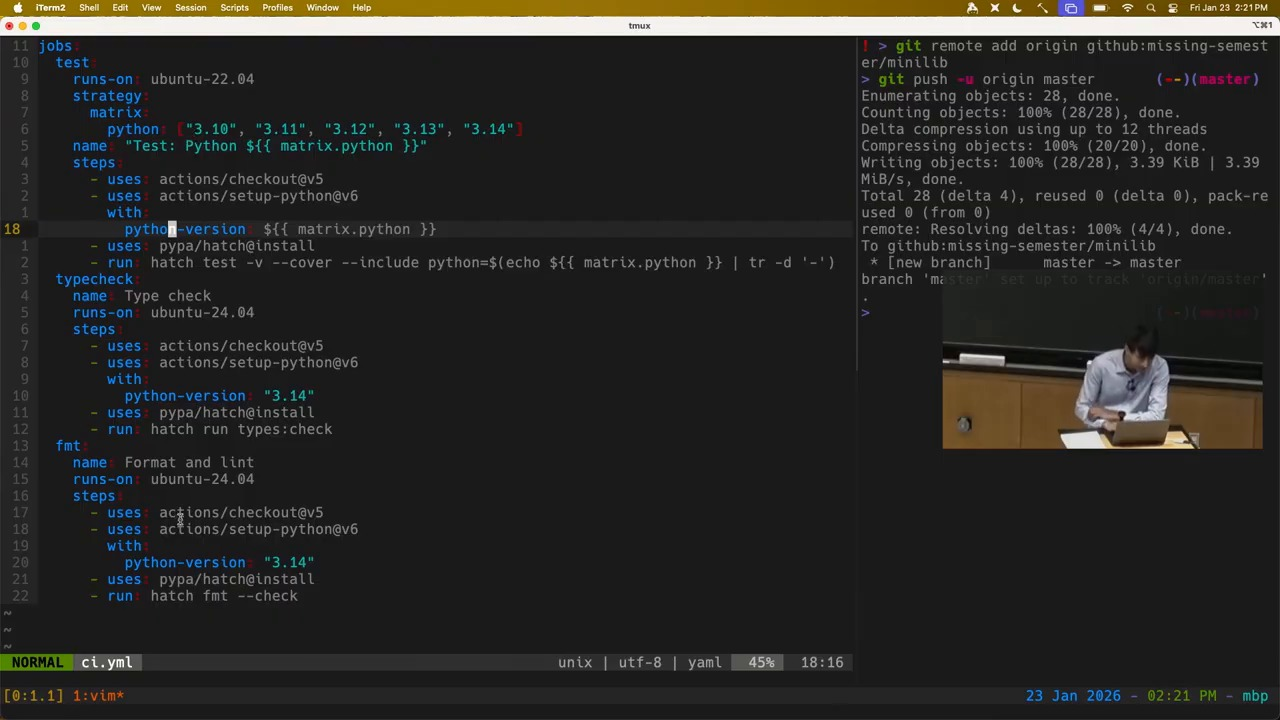
\includegraphics[width=0.92\textwidth]{figures/fig_18_gha_yaml.jpg}
\caption{GitHub Actions 的 workflow 文件定义了触发事件、Python 版本矩阵和几个任务\vtag}
\end{figure}
\srcnote{00:45:30--00:45:45}
\end{minipage}


GitHub Actions 通过一个特殊目录配置：\texttt{.github/workflows}，所有 workflow 都放在里面。讲者先在 missing-semester 组织下新建了一个公开仓库，添加远程并推送，让 CI 在后台运行，同时讲解配置。这个配置只有一个文件，有几个值得看的部分：
\begin{itemize}
\item 触发事件：每当推送修改、有人发起拉取请求，或者按计划（有一种可以查到的特定语法）自动运行检查。按计划运行有助于确保代码与所有外部依赖兼容：如果某个依赖做了破坏性修改，定时运行 CI 能帮你发现；虽然不是你的错，别人造成了问题，你还是得想办法修好。
\item 任务（jobs）：配置写在 YAML 文件中，这是一种声明式的配置文件，语法可以在 GitHub 文档中查到，其他 CI 服务也类似。这里定义了一个要在多个 Python 版本上运行的测试矩阵，还有测试任务、类型检查任务和格式检查任务。
\item 步骤：可以指定运行的操作系统；GitHub Actions 是可组合的，可以建立在别的 action 之上，比如检出仓库的最新提交、在机器上安装 Python、安装 Hatch；最后基本上就是定义一条要运行的 shell 命令，只要有一步返回非零退出码，CI 服务就判定失败。
\end{itemize}

\begin{lstlisting}[language=bash]
# .github/workflows/ci.yml (sketch)
on:
  push:
  pull_request:
  schedule:
    - cron: "0 9 * * 1"
jobs:
  test:
    runs-on: ubuntu-latest
    strategy:
      matrix:
        python-version: ["3.10", "3.11", "3.12", "3.13", "3.14"]
    steps:
      - uses: actions/checkout@v4
      - uses: actions/setup-python@v5
        with:
          python-version: ${{ matrix.python-version }}
      - run: pip install hatch
      - run: hatch test
\end{lstlisting}

\begin{warningbox}{示意配置}
讲义作者提醒：上面的 YAML 是讲义作者按讲者描述的结构写的简化示意，并非讲者仓库中的原文件；其中的定时表达式表示每周一 9 点（GitHub Actions 的定时按 UTC 计算）。实际配置请以 GitHub Actions 文档为准。
\end{warningbox}

\noindent\begin{minipage}{\textwidth}
\begin{figure}[H]
\centering
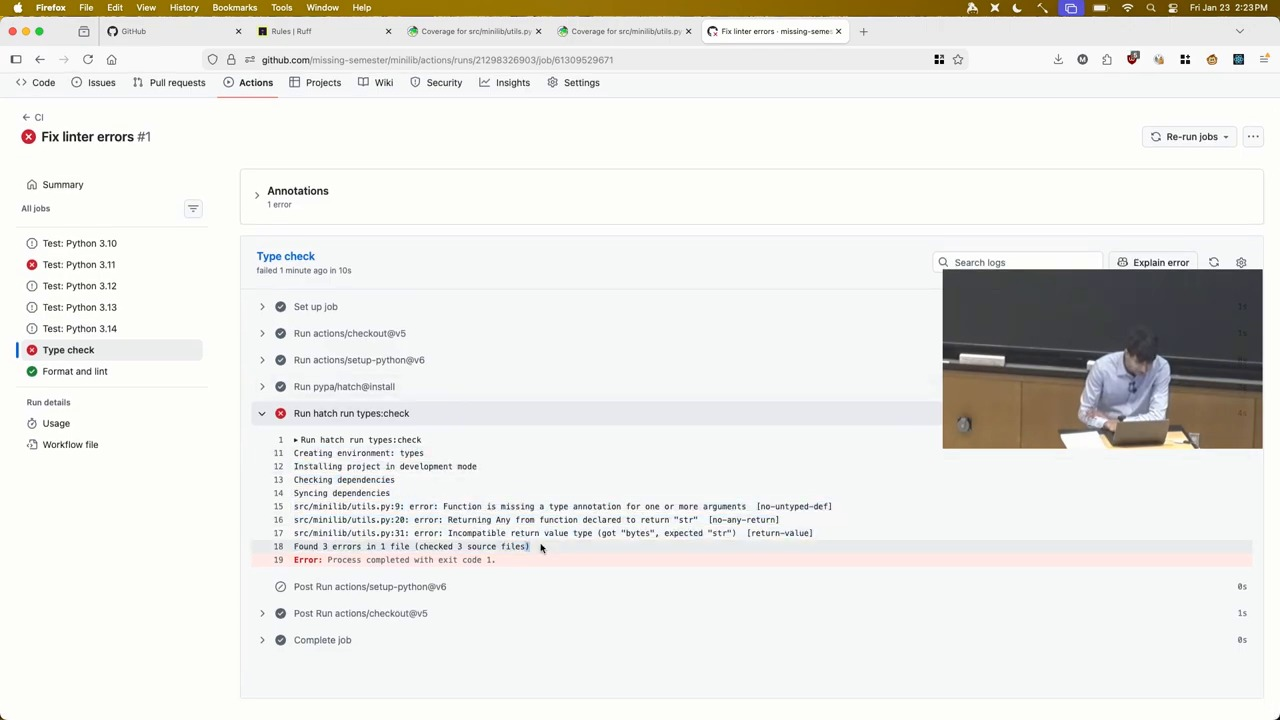
\includegraphics[width=0.92\textwidth]{figures/fig_19_gha_results.jpg}
\caption{在 Actions 页面可以看到每个任务的结果，这次类型检查任务失败了\vtag}
\end{figure}
\srcnote{00:46:45--00:47:00}
\end{minipage}


刷新 GitHub 上仓库的 Actions 标签页，可以看到最新提交的格式检查和 linter 通过了，有绿色对勾，但类型检查器失败了，点进去能看到类型检查器的详细输出。接下来就可以迭代：哪里失败就去修，在本机测试，推送到 CI 确认通过，直到一切正常。

\subsection{对拉取请求尤其有用}

Jon 补充说，CI 对来自他人的拉取请求特别有用：很多给你的项目做贡献的人，连运行格式化工具、类型检查器这种基本的事都不做，CI 会强制替他们运行；而 CI 是否通过的信息会直接附在 GitHub 的拉取请求上，一眼就能看到。

\subsection{持续部署}

与持续集成密切相关的概念是持续部署（CD）。很多项目不仅用 CI 基础设施测试代码，还用它部署：如果你在做二进制软件，可以运行编译器为所有不同的操作系统生成构建并自动发布到网上；也可以自动把应用部署到 Web 服务上。Missing Semester 自己就在用：课程仓库通过 CI 和 GitHub Pages，在每次推送讲义仓库时自动发布更新后的网站。

有同学问持续集成到底是什么。讲者总结：它是在仓库发生某些事情时在云端运行代码的方式，可以做很多事，最常见的就是运行这些代码质量检查：格式检查、linter、测试，还可以计算代码覆盖率并上传到 Codecov 这样的服务，在网页上长期监控覆盖率的变化。基本上可以运行任何你想要的代码，写自己的脚本也行，代码质量只是主要用途之一。

\subsection{本章小结}

CI 在推送、拉取请求或定时触发时，在远程机器上运行格式检查、linter、类型检查和测试，并可以用矩阵覆盖多个平台和语言版本；结果附在拉取请求上，对外部贡献尤其有用；CD 进一步用同一套设施自动构建和发布。

\section{命令运行器}

讲者说，这节课大家看到他一直在敲 \texttt{hatch fmt}、\texttt{hatch test} 这样的命令，它们是怎么工作的？Hatch 是一个 Python 项目管理工具，支持 \texttt{pyproject.toml} 配置文件，也内置了很多东西，比如 \texttt{hatch fmt} 是内置命令，底层使用 Ruff 格式化工具和 linter。这让你可以方便地运行所有与代码质量相关的命令，而不用敲很长的调用。

但在某些项目中，如果没有用语言特定的项目管理工具，你可能得敲类似 \texttt{mypy -{}-strict -{}-install-types -{}-non-interactive src tests} 这样的命令来对代码运行类型检查器。每次都敲这个很烦，于是就有了命令运行器（command runner）的概念：基本上就是一份命令列表。

\noindent\begin{minipage}{\textwidth}
\begin{figure}[H]
\centering
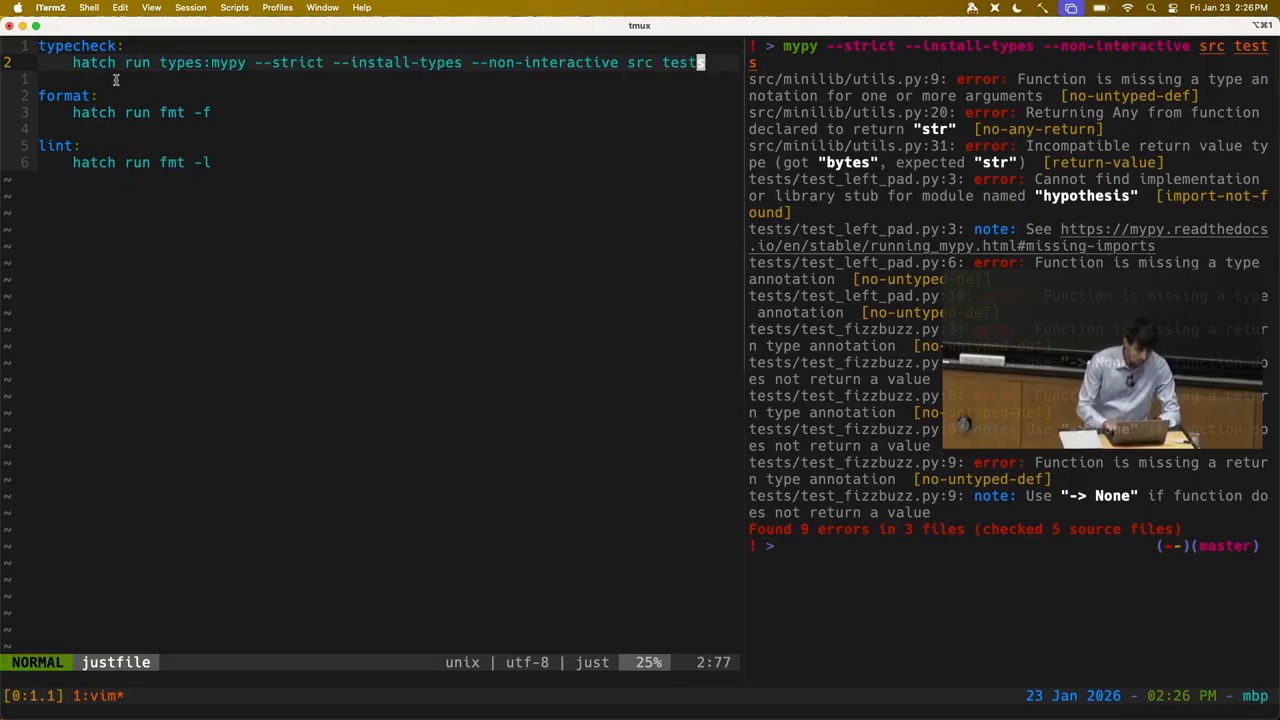
\includegraphics[width=0.92\textwidth]{figures/fig_20_justfile.jpg}
\caption{justfile 为常用的长命令定义简短的别名\vtag}
\end{figure}
\srcnote{00:50:15--00:50:30}
\end{minipage}


讲者展示了一个叫 just 的命令运行器：可以为较长的命令定义简短的别名。他说在这里有点多余，因为 Hatch 也支持这种功能；但如果项目没有用类似工具，又不想每次都敲那么长的字符串，就可以运行 \texttt{just typecheck}、\texttt{just format} 等，它会执行 justfile 中定义的命令。

\begin{lstlisting}[language=bash]
# justfile (sketch)
typecheck:
    mypy --strict --install-types --non-interactive src tests

format:
    ruff format .

test:
    pytest
\end{lstlisting}

\begin{knowledgebox}{命令运行器的好处}
讲义作者补充：把常用命令写进 justfile（或 Makefile、\texttt{pyproject.toml} 的脚本段）有三个好处：新成员不用记长命令；本地、pre-commit 钩子和 CI 可以调用同一个入口，保证三处运行的检查一致；编程智能体也可以读这个文件，知道项目该怎样格式化、检查和测试。
\end{knowledgebox}

\section{附加主题：正则表达式}

\subsection{正则表达式用在哪里}

讲完代码质量后，讲者又花了大约 10 分钟讲正则表达式。这个话题原本在开发环境那一讲，因为时间原因挪了过来，它是跨领域的，放在这里也合适。正则表达式（regular expression，常缩写为 regex）是一种描述字符串集合、或者说字符串模式的语言。它常用于命令行工具中接收字符串模式的参数，比如本讲给 \texttt{ag} 的模式；又如你写了几千个测试，只想运行其中一部分，\texttt{hatch test} 这类工具就支持传入一个正则表达式，只运行名字匹配的测试。

\noindent\begin{minipage}{\textwidth}
\begin{figure}[H]
\centering
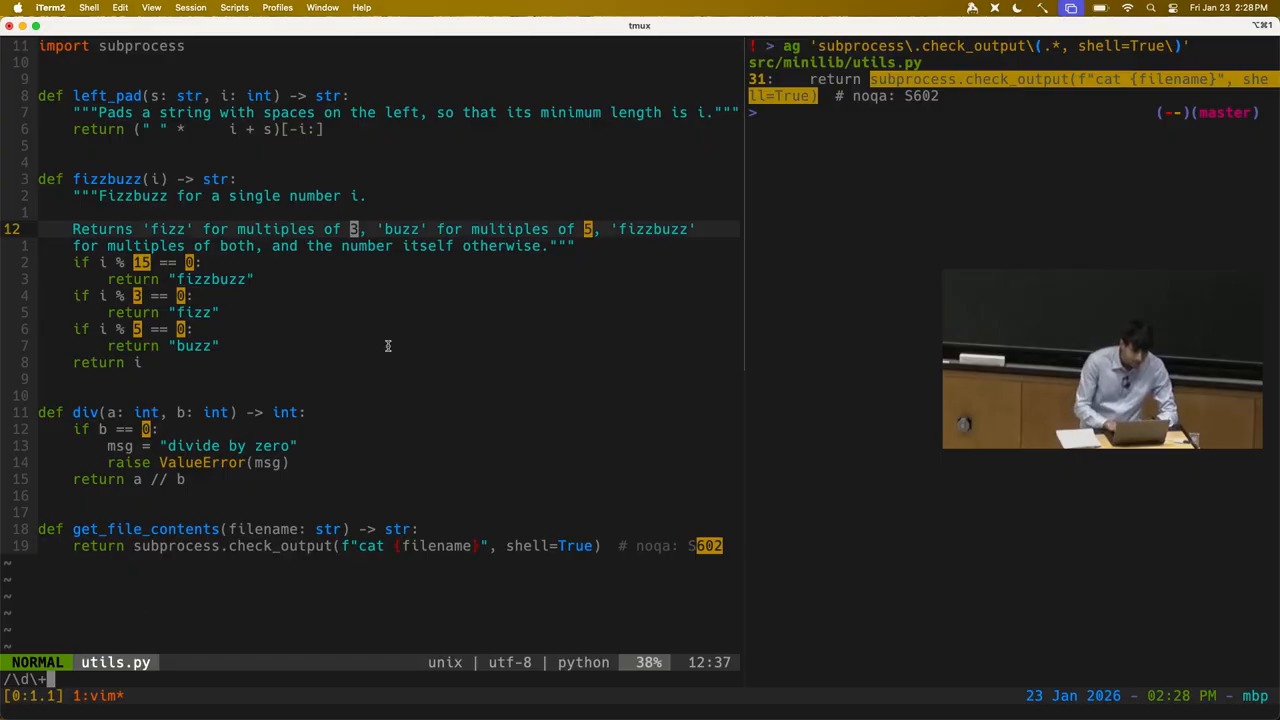
\includegraphics[width=0.92\textwidth]{figures/fig_21_vim_regex.jpg}
\caption{在 Vim 中用正则表达式搜索，所有数字都被高亮出来\vtag}
\end{figure}
\srcnote{00:52:30--00:52:45}
\end{minipage}


另一个用途是在 IDE 中按正则表达式搜索：讲者在 \texttt{utils.py} 中搜索所有数字，用 Vim 的正则语法写作 \texttt{\textbackslash{}d\textbackslash{}+}，代码里的所有数字都被高亮。还可以搜索替换，比如把所有匹配替换成 hi，虽然没什么用，但能看到它们全被替换了。所以正则表达式对搜索替换也很有用。

\subsection{理论概念与不同的“方言”}

讲者提醒，正则表达式本是一个计算机科学理论中的概念，而许多编程语言和工具中都有它的实现：他的 Vim 编辑器有一套实现，\texttt{ag} 也有一套。有点烦人的是，正则表达式有很多“方言”（flavor）：底层概念相同，表层语法略有差异。比如 Vim 中要写 \texttt{\textbackslash{}d\textbackslash{}+}，两个特殊符号前都要加反斜杠；而在 \texttt{ag} 中写 \texttt{\textbackslash{}d+} 就行。这些小差异要么记住，要么用的时候查。讲义里链接了一份完整的正则语法指南，建议找时间浏览一遍。

\subsection{在 regex101 上逐个试验}

讲者推荐使用 regex101.com 这类网站：可以写下一堆测试字符串，再写一个正则表达式，它会显示哪些字符串被匹配，并解释这个表达式；还能在不同方言间切换，比如 Python 和 JavaScript 的正则略有不同。有同学问测试字符串是不是相当于代码，讲者说可以是代码，也可以是任何你想匹配的东西；更抽象地说，正则表达式是描述字符串集合的语言，这里显示的是哪些具体字符串属于这个集合。

\noindent\begin{minipage}{\textwidth}
\begin{figure}[H]
\centering
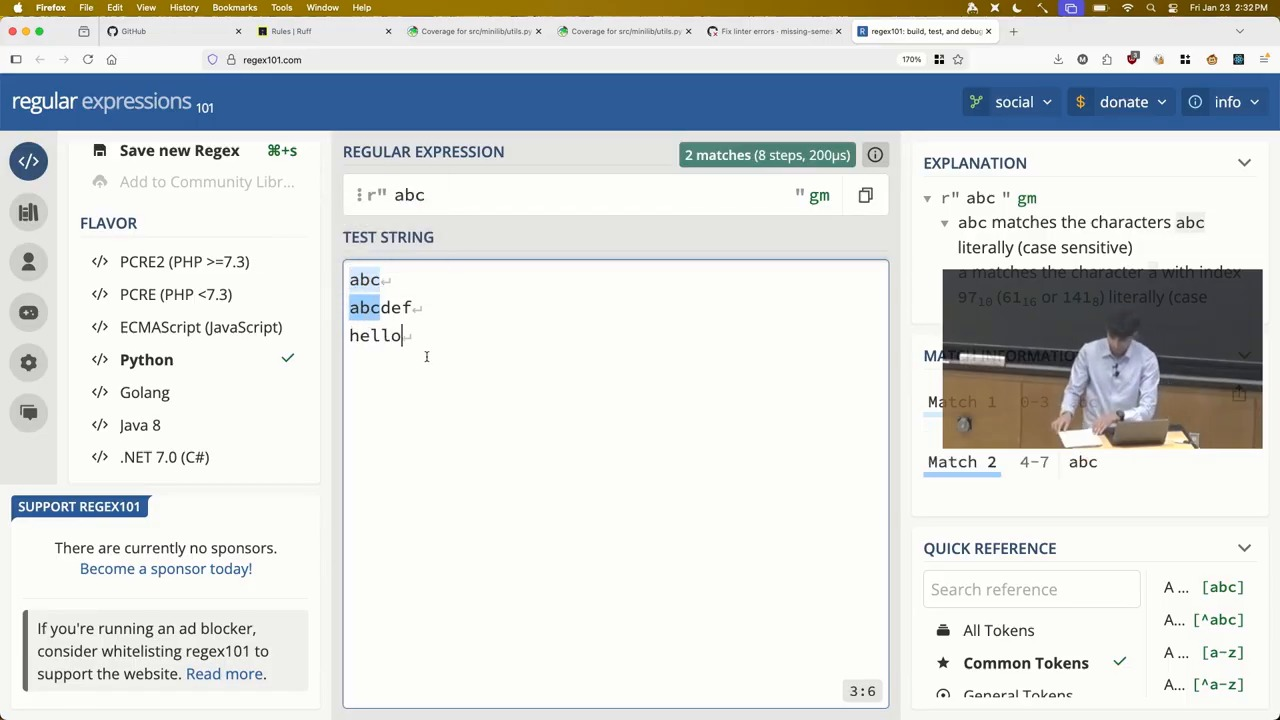
\includegraphics[width=0.92\textwidth]{figures/fig_22_regex101.jpg}
\caption{在 regex101 上，普通字符组成的模式只匹配同样的字面字符串\vtag}
\end{figure}
\srcnote{00:56:15--00:56:30}
\end{minipage}


\begin{importantbox}{正则表达式的基本构件}
讲者在 regex101 上逐个演示了这些构件：
\begin{itemize}
\item 字面字符：模式 \texttt{abc} 只匹配字面的 abc，这是最基本的构件。
\item 字符类：\texttt{[abc]} 匹配 a、b、c 中的任意一个字符；可以组合，\texttt{hello[abc]} 匹配 hello a、hello b，但不匹配 hello d。可以用范围，如 \texttt{[a-f]}。
\item 否定字符类：\texttt{[\^{}abc]} 匹配不在其中的任意一个字符。
\item 选择：\texttt{hello|world} 匹配左边或右边的模式。
\item 转义类：\texttt{\textbackslash{}d} 匹配数字，\texttt{\textbackslash{}w} 匹配单词字符，\texttt{\textbackslash{}b} 匹配单词边界。
\item 点号 \texttt{.} 匹配任意字符；\texttt{\textbackslash{}\textbackslash{}} 匹配字面的反斜杠。
\item 锚点：\texttt{\^{}} 匹配行首，\texttt{\$} 匹配行尾。
\item 量词：\texttt{+} 表示前面的东西出现一次或多次，\texttt{\{4\}} 表示恰好出现 4 次。
\item 分组：圆括号既用于分组、控制运算优先级，也是捕获组。
\end{itemize}
\end{importantbox}

\noindent\begin{minipage}{\textwidth}
\begin{figure}[H]
\centering
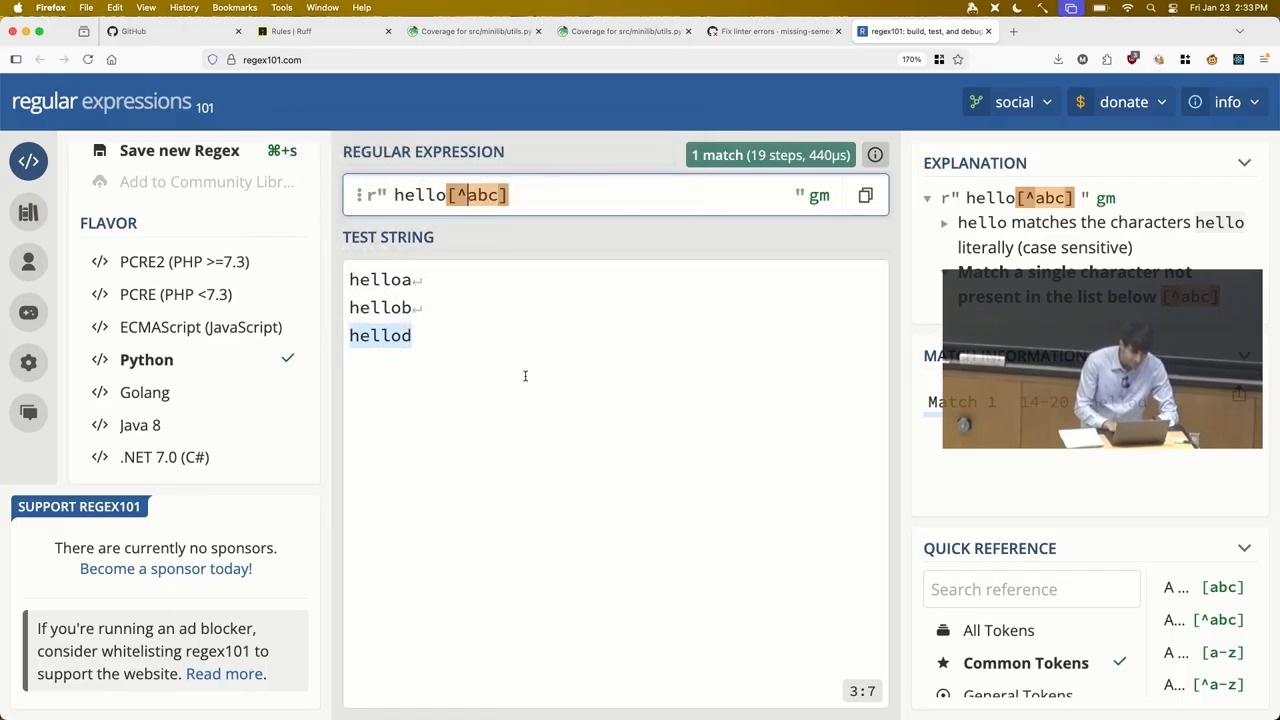
\includegraphics[width=0.92\textwidth]{figures/fig_23_regex_neg.jpg}
\caption{字符类后面跟着具体字符时，只匹配其中列出的那几个字符之一\vtag}
\end{figure}
\srcnote{00:57:00--00:57:15}
\end{minipage}


有同学问 \texttt{hello[\^{}abc]} 能否匹配 “hello ab”。在 regex101 上一试，不能：从左边开始匹配，hello 匹配到这里，下一个字符必须不是 a、b、c 中的任何一个，而它是 a，所以不满足。方括号中描述的永远是“一个”字符。

\noindent\begin{minipage}{\textwidth}
\begin{figure}[H]
\centering
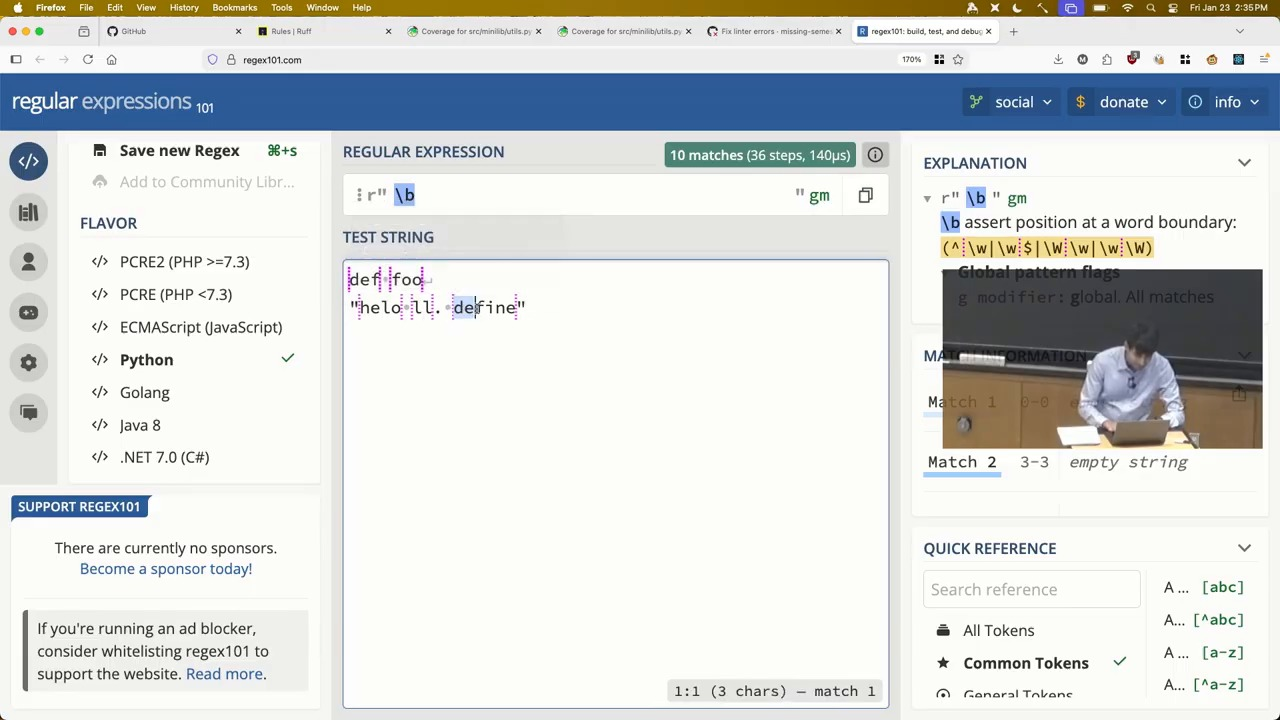
\includegraphics[width=0.92\textwidth]{figures/fig_24_regex_b.jpg}
\caption{用单词边界把 def 关键字和 define 中的 def 区分开\vtag}
\end{figure}
\srcnote{00:59:00--00:59:15}
\end{minipage}


讲者特别介绍了很方便的 \texttt{\textbackslash{}b}：假设要找出 Python 代码中所有的函数定义，即所有的 def，但 def 也可能出现在别的上下文中，比如字符串里的 define。可以写 \texttt{\textbackslash{}bdef\textbackslash{}b}：单词边界匹配的是字符之间的位置，而不是字符本身。这样就只匹配独立的 def，不匹配 define 中的 def。

\subsection{捕获组与搜索替换}

讲者说，分组不仅用于分组和运算优先级，还是捕获组，在搜索替换中可以引用匹配到的子部分。他举了一个“古怪”的例子：在 Vim 中把所有数字替换成重复两遍的自己，比如 15 变成 1515，0 变成 00。Vim 中捕获组需要转义，写作 \texttt{\textbackslash{}(\textbackslash{}d\textbackslash{}+\textbackslash{})}，替换部分用 \texttt{\textbackslash{}1} 引用第一个捕获组，写成 \texttt{\textbackslash{}1\textbackslash{}1}，再加 \texttt{/g} 全局替换。Vim 会预览替换，按回车后 15 变成了 1515。讲者说实际中可以想出更有意义的例子，这种带捕获组的正则加替换模式，在 IDE 等场合很有用。

\noindent\begin{minipage}{\textwidth}
\begin{figure}[H]
\centering
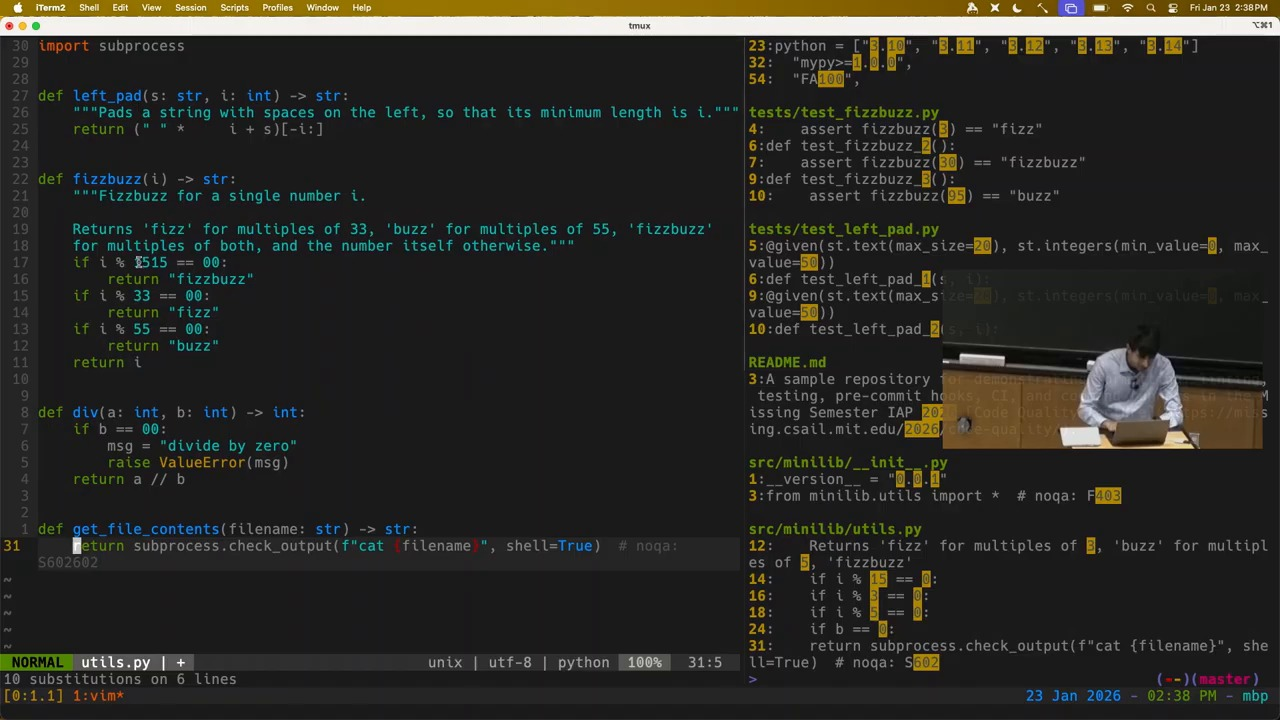
\includegraphics[width=0.92\textwidth]{figures/fig_25_vim_capture.jpg}
\caption{Vim 的替换命令用反斜杠加数字引用捕获组，把每个数字重复一遍\vtag}
\end{figure}
\srcnote{01:02:30--01:02:45}
\end{minipage}


\begin{lstlisting}[language=bash]
:%s/\d\+/hi/g            " replace every number with "hi"
:%s/\(\d\+\)/\1\1/g      " repeat every number: 15 -> 1515
\end{lstlisting}

\subsection{在程序中使用正则表达式}

\noindent\begin{minipage}{\textwidth}
\begin{figure}[H]
\centering
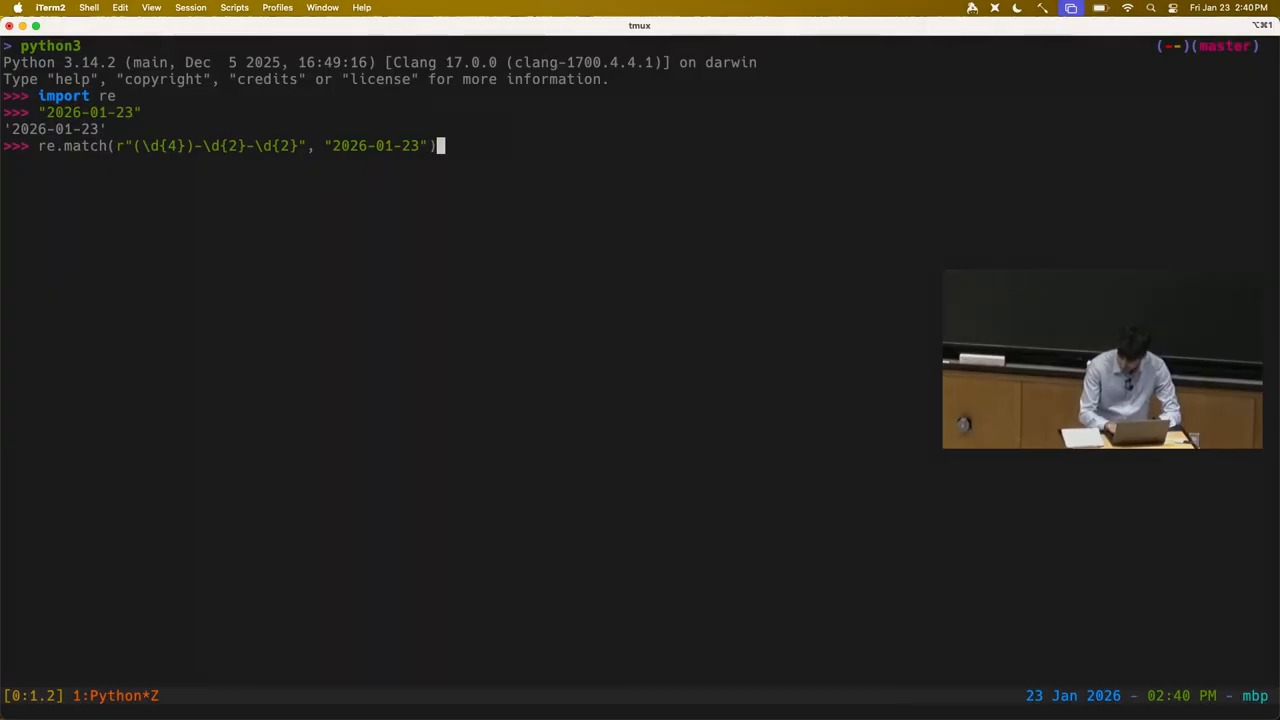
\includegraphics[width=0.92\textwidth]{figures/fig_26_python_re.jpg}
\caption{在 Python 中用 re.match 和捕获组从日期字符串中取出年份\vtag}
\end{figure}
\srcnote{01:04:00--01:04:15}
\end{minipage}


写程序时也经常需要描述字符串模式，比如解析电子邮件地址。讲者举例：要解析一个文件，里面有很多 YYYY-MM-DD 格式的日期，比如那天的日期 2026-01-23，想取出年份。在 Python 中可以用 \texttt{re.match}，字符串前加 \texttt{r} 表示原始字符串，少写很多转义；\texttt{\textbackslash{}d\{4\}} 表示四个数字，放进捕获组，后面跟着两个数字、再两个数字。把结果绑定到 \texttt{m}，\texttt{m.group(1)} 就是第一个捕获组；定义多个捕获组就能取出各个部分。讲者说这对分析 Web 服务器日志之类的任务很有用，比如找出访问服务器的 IP 地址：写一个正则表达式，用编程语言的正则库过滤，或者把同样的模式交给 grep。

\begin{lstlisting}[language=Python]
import re

m = re.match(r"(\d{4})-(\d{2})-(\d{2})", "2026-01-23")
m.group(1)    # '2026'
m.groups()    # ('2026', '01', '23')
\end{lstlisting}

\subsection{正则表达式的局限}

讲者总结：正则表达式是描述字符串集合的非常紧凑的语言，但有局限，讲义里链接了一些相关的计算机科学理论。基本上，有些事情不能用正则表达式做，比如正确解析 HTML，正则表达式的表达能力不够，这时需要更复杂的解析器。但对很多字符串处理任务来说，正则表达式非常好用，简单、简洁，比完整的上下文无关文法解析器轻量得多。

有同学问能否在自己的代码里用正则表达式。讲者说当然可以，刚才在 Python REPL 里就是这么做的，在程序里 \texttt{import re} 即可。很多工具，比如 \texttt{ag}，也是用外部依赖实现正则，它用的是一个流行的 Rust 正则库，并没有自己造轮子。Python 中叫 \texttt{re}，Rust 中则是一个流行的第三方库，不在标准库里，取决于语言。

\begin{knowledgebox}{为什么正则表达式解析不了 HTML}
讲义作者补充：理论上，正则表达式描述的是“正则语言”，可以用有限状态自动机识别，而有限状态机没有无限的记忆，无法数清任意深度的嵌套。HTML 的标签可以任意嵌套，需要配对，这超出了正则语言的能力，需要上下文无关文法和栈。实际工具中的“正则”常带有反向引用等扩展，能力超出理论上的正则语言，但用它们解析嵌套结构依然脆弱，应当使用专门的解析器。
\end{knowledgebox}

\begin{practicebox}{正则练习}
讲义作者整理：在 regex101 上依次写出以下模式并用几个字符串验证：匹配整行只有 world 的行；匹配 Python 函数定义行开头的 \texttt{def} 关键字但不匹配 define；从形如 \texttt{2026-01-23} 的字符串中用捕获组取出月份；然后在编辑器里用捕获组把 \texttt{YYYY-MM-DD} 改写成 \texttt{DD/MM/YYYY}。
\end{practicebox}

\section{课程结束后的答疑}

讲完正则表达式，讲者说这就是今天以及整门课的全部内容，欢迎大家就整门课的任何内容提问，并请 Jon 也上来一起回答。

\subsection{去哪里找提示词}

有同学问去哪里找好的提示词。Jon 说，LLM 很擅长遵循英语指令，不需要以特别的方式写提示；有时用一些办法让它关注特定的东西、使用特定的关键词，可以多榨出一点效果，但那是最后几个百分点，而不是大部分价值所在。网上有很多资源，有人会在 AI 辅助编程的提交信息中附上提示词。讲者补充说，没有一个汇总所有提示词的仓库；网上有很多关于如何写好提示词的文章和视频，OpenAI、Anthropic 等开发模型的实验室也写了相当好的一手指南，因为他们希望你用好他们的产品。示例提示词比较少见，因为示例往往与具体代码库和具体任务紧密相关；想看示例，最好的办法也许是找人录下的与智能体协作的视频，或者在 Bluesky、Mastodon、LinkedIn、Twitter 上找人分享的经验，但命中率可能很低，还是指南类文章更好。

\subsection{测试应该放在哪里}

有同学问测试和代码分开放是不是一个基本原则。Jon 说不是：比如在 Rust 中，把单元测试和被测函数写在同一个文件里很常见，因为 Rust 的单元测试往往很小；写更复杂的集成测试时，Rust 也有单独的机制把它们放在单独的文件里，就像这里的 Python 一样。讲者补充 Python 也有类似的 doctest，可以把测试写在代码旁边。Jon 说，这取决于测试是小到适合放在函数旁边，还是复杂到需要拆分出来。对编译型语言，这个区别还会影响构建：如果单元测试和代码在同一个文件里，改了测试就可能导致重新编译，因为变更跟踪是基于文件的，而不是基于文件中哪一部分被修改。

\subsection{怎样测试调用外部 API 的代码}

有同学问，程序里有大量 API 调用时怎么测试。讲者说有几种方法：
\begin{itemize}
\item 模拟（mocking）：为应用依赖的组件构建模拟版本，在测试运行时注入。比如你在做一个 AI 智能体，里面有调用 OpenAI API 的客户端，可以模拟这个客户端，为特定测试中的特定参数伪造返回值。Jon 解释：模拟就是实现某个东西的 API，但背后是你自己的实现，比如实现一个与 YouTube API 接口相同的程序，背后只是你写的简单实现，测试时让程序指向它而不是真正的 YouTube API。这样你能更严格地控制背后发生的事：让它返回错误或任何你想要的结果，也可以在没有网络连接时运行。
\item 录制与回放：对真实 API 运行一次测试，录下所有网络通信，以后的测试回放这些记录。讲者说 Python 中有一个库叫 pytest-vcr 之类的名字。
\item 直接对真实 API 运行测试：这也是人们会做的事，有利有弊。
\end{itemize}

\begin{lstlisting}[language=Python]
from unittest.mock import MagicMock

def test_summarize_uses_client():
    client = MagicMock()
    client.complete.return_value = "a short summary"
    assert summarize(client, "long text") == "a short summary"
    client.complete.assert_called_once()
\end{lstlisting}

\begin{warningbox}{示例中的函数是虚构的}
讲义作者提醒：上面的 \texttt{summarize} 函数和 \texttt{client.complete} 方法是讲义作者为说明“注入模拟客户端”这一思路而虚构的；\texttt{MagicMock} 来自 Python 标准库的 \texttt{unittest.mock}。
\end{warningbox}

最后讲者感谢大家，开玩笑说希望下次再见不用等六年。

\section{总结}

\begin{itemize}
\item 代码质量的概念几乎是通用的，工具是语言特定的：记住概念，用到时查具体工具。
\item 格式化工具自动处理表层语法，可只检查或直接修复；EditorConfig 统一不同编辑器的基本设置。
\item linter 做静态的语义分析，能自动修复其中安全的部分；误报用 \texttt{noqa} 按行关闭；规则文档能教你写更好的代码；项目特定规则可以用 semgrep 在语法树层面编写。
\item 测试分单元、集成、功能等粒度；失败的测试给出具体反例；覆盖率指出没测到的代码，但高覆盖率不等于好测试，AI 写的测试要审查。
\item 性质测试写下部分规格，自动生成输入并给出反例；记得写 \texttt{assert}。
\item pre-commit 钩子在提交前运行检查；CI 在远程机器上按事件运行检查和测试矩阵，结果附在拉取请求上；CD 自动构建和发布。
\item 命令运行器为长命令提供简短入口。
\item 正则表达式是描述字符串集合的紧凑语言，有多种方言；捕获组可用于搜索替换和程序中的解析；它无法处理任意嵌套的结构。
\end{itemize}

\begin{practicebox}{自测}
\begin{enumerate}
\item 格式化工具和 linter 的区别是什么？为什么有些格式化工具几乎不可配置？
\item 什么时候应该用 \texttt{noqa}？为什么 \texttt{shell=True} 危险？
\item 为什么用正则表达式查找特定函数调用很脆弱，semgrep 怎样解决这个问题？
\item 覆盖率 100\% 是否意味着没有 bug？举例说明。
\item 为 \texttt{left\_pad} 再写一条性质，使得“直接返回原字符串”的错误实现无法通过。
\item 有了 pre-commit 钩子，为什么还需要 CI？
\end{enumerate}
\end{practicebox}

\end{document}
